%%%%%%%%%%%%%%%%%%%%%%%%%%%%%%%%%%%%%%%%%%%%%%
%
%		My Thesis
%
%		EDOC Template
%		2011
%
%%%%%%%%%%%%%%%%%%%%%%%%%%%%%%%%%%%%%%%%%%%%%%


%%%%%%%%%%%%%%%%%%%%%%%%%%%%%%%%%%%%%%%%%%%%%%
%
%		Thesis Settings
%
%		EDOC Template
%		2011
%
%%%%%%%%%%%%%%%%%%%%%%%%%%%%%%%%%%%%%%%%%%%%%%
\documentclass[a4paper,11pt,fleqn]{book}
%\documentclass[a4paper,11pt,fleqn,draft]{book}
\usepackage[T1]{fontenc}
\usepackage[utf8]{inputenc}
\usepackage[french,german,english]{babel}


%%%%%%%%%%%%%%%%%%%%%%%%%%%%%%%%%%%%%%%%%%%%%%%
%% EDOC THESIS TEMPLATE: Variant 1.0 -> Latin modern, large text width&height
%%%%%%%%%%%%%%%%%%%%%%%%%%%%%%%%%%%%%%%%%%%%%%%
\usepackage{lmodern}
%\usepackage[a4paper,top=22mm,bottom=28mm,inner=35mm,outer=25mm]{geometry}
\usepackage[a4paper,top=32mm,bottom=28mm,inner=35mm,outer=25mm]{geometry}
%%%%%%%%%%%%%%%%%%%%%%%%%%%%%%%%%%%%%%%%%%%%%%%

%%%%%%%%%%%%%%%%%%%%%%%%%%%%%%%%%%%%%%%%%%%%%%
% EDOC THESIS TEMPLATE: Variant 2.0 -> Utopia, Gabarrit A (lighter pages)
%%%%%%%%%%%%%%%%%%%%%%%%%%%%%%%%%%%%%%%%%%%%%%
%\usepackage{fourier} % Utopia font-typesetting including mathematical formula compatible with newer TeX-Distributions (>2010)
%\usepackage{utopia} % on older systems -> use this package instead of fourier in combination with mathdesign for better looking results
%\usepackage[adobe-utopia]{mathdesign}
%\setlength{\textwidth}{146.8mm} % = 210mm - 37mm - 26.2mm
%\setlength{\oddsidemargin}{11.6mm} % 37mm - 1in (from hoffset)
%\setlength{\evensidemargin}{0.8mm} % = 26.2mm - 1in (from hoffset)
%\setlength{\topmargin}{-2.2mm} % = 0mm -1in + 23.2mm
%\setlength{\textheight}{221.9mm} % = 297mm -29.5mm -31.6mm - 14mm (12 to accomodate footline with pagenumber)
%\setlength{\headheight}{14pt}
%%%%%%%%%%%%%%%%%%%%%%%%%%%%%%%%%%%%%%%%%%%%%%



\setlength{\parindent}{0pt}

\usepackage{setspace} % increase interline spacing slightly
\setstretch{1.1}

\makeatletter
\setlength{\@fptop}{0pt}  % for aligning all floating figures/tables etc... to the top margin
\makeatother


\usepackage{graphicx,xcolor}
\graphicspath{{images/}}

\usepackage{subfig}
\usepackage{booktabs}
\usepackage{lipsum}
\usepackage{microtype}
\usepackage{url}
\usepackage[final]{pdfpages}

\usepackage{fancyhdr}
\renewcommand{\sectionmark}[1]{\markright{\thesection\ #1}}
\pagestyle{fancy}
	\fancyhf{}
	\renewcommand{\headrulewidth}{0.4pt}
	\renewcommand{\footrulewidth}{0pt}
	\fancyhead[OR]{\bfseries \nouppercase{\rightmark}}
	\fancyhead[EL]{\bfseries \nouppercase{\leftmark}}
	\fancyfoot[EL,OR]{\thepage}
\fancypagestyle{plain}{
	\fancyhf{}
	\renewcommand{\headrulewidth}{0pt}
	\renewcommand{\footrulewidth}{0pt}
	\fancyfoot[EL,OR]{\thepage}}
\fancypagestyle{addpagenumbersforpdfimports}{
	\fancyhead{}
	\renewcommand{\headrulewidth}{0pt}
	\fancyfoot{}
	\fancyfoot[RO,LE]{\thepage}
}

\usepackage{listings}
\lstset{language=[LaTeX]Tex,tabsize=4, basicstyle=\scriptsize\ttfamily, showstringspaces=false, numbers=left, numberstyle=\tiny, numbersep=10pt, breaklines=true, breakautoindent=true, breakindent=10pt}

% HYP REF LINK IN PDF
\usepackage{hyperref}
\hypersetup{pdfborder={0 0 0},
	colorlinks=true,
	linkcolor=red,
	citecolor=red,
	urlcolor=blue}
\urlstyle{same}

\makeatletter
\def\cleardoublepage{\clearpage\if@twoside \ifodd\c@page\else
    \hbox{}
    \thispagestyle{empty}
    \newpage
    \if@twocolumn\hbox{}\newpage\fi\fi\fi}
\makeatother \clearpage{\pagestyle{plain}\cleardoublepage}


%%%%% CHAPTER HEADER %%%%
\usepackage{color}
\usepackage{tikz}
\usepackage[explicit]{titlesec}
\newcommand*\chapterlabel{}
%\renewcommand{\thechapter}{\Roman{chapter}}
\titleformat{\chapter}[display]  % type (section,chapter,etc...) to vary,  shape (eg display-type)
	{\normalfont\bfseries\Huge} % format of the chapter
	{\gdef\chapterlabel{\thechapter\ }}     % the label
 	{0pt} % separation between label and chapter-title
 	  {\begin{tikzpicture}[remember picture,overlay]
    \node[yshift=-8cm] at (current page.north west)
      {\begin{tikzpicture}[remember picture, overlay]
        \draw[fill=black] (0,0) rectangle(35.5mm,15mm);
        \node[anchor=north east,yshift=-7.2cm,xshift=34mm,minimum height=30mm,inner sep=0mm] at (current page.north west)
        {\parbox[top][30mm][t]{15mm}{\raggedleft $\phantom{\textrm{l}}$\color{white}\chapterlabel}};  %the black l is just to get better base-line alingement
        \node[anchor=north west,yshift=-7.2cm,xshift=37mm,text width=\textwidth,minimum height=30mm,inner sep=0mm] at (current page.north west)
              {\parbox[top][30mm][t]{\textwidth}{\color{black}#1}};
       \end{tikzpicture}
      };
   \end{tikzpicture}
   \gdef\chapterlabel{}
  } % code before the title body

\titlespacing*{\chapter}{0pt}{50pt}{80pt} % LDP : change 30pt to 80pt after margin to avoid collision for not numbered chapters
\titlespacing*{\section}{0pt}{13.2pt}{*0}  % 13.2pt is line spacing for a text with 11pt font size
\titlespacing*{\subsection}{0pt}{13.2pt}{*0}
\titlespacing*{\subsubsection}{0pt}{13.2pt}{*0}

\newcounter{myparts}
\newcommand*\partlabel{}
\titleformat{\part}[display]  % type (section,chapter,etc...) to vary,  shape (eg display-type)
	{\normalfont\bfseries\Huge} % format of the part
	{\gdef\partlabel{\thepart\ }}     % the label
 	{0pt} % separation between label and part-title
 	  {\setlength{\unitlength}{20mm}
	  \addtocounter{myparts}{1}
	  \begin{tikzpicture}[remember picture,overlay]
    \node[anchor=north west,xshift=-65mm,yshift=-6.9cm-\value{myparts}*20mm] at (current page.north east) % for unknown reasons: 3mm missing -> 65 instead of 62
      {\begin{tikzpicture}[remember picture, overlay]
        \draw[fill=black] (0,0) rectangle(62mm,20mm);   % -\value{myparts}\unitlength
        \node[anchor=north west,yshift=-6.1cm-\value{myparts}*20mm,xshift=-60.5mm,minimum height=30mm,inner sep=0mm] at (current page.north east)
        {\parbox[top][30mm][t]{55mm}{\raggedright \color{white}Part \partlabel $\phantom{\textrm{l}}$}};  %the phantom l is just to get better base-line alingement
        \node[anchor=north east,yshift=-6.1cm-\value{myparts}*20mm,xshift=-63.5mm,text width=\textwidth,minimum height=30mm,inner sep=0mm] at (current page.north east)
              {\parbox[top][30mm][t]{\textwidth}{\raggedleft \color{black}#1}};
       \end{tikzpicture}
      };
   \end{tikzpicture}
   \gdef\partlabel{}
  } % code before the title body

\usepackage{amsmath}
% Fix the problem with delimiter size caused by fourier and amsmath packages.
\makeatletter
\def\resetMathstrut@{%
  \setbox\z@\hbox{%
    \mathchardef\@tempa\mathcode`\(\relax
      \def\@tempb##1"##2##3{\the\textfont"##3\char"}%
      \expandafter\@tempb\meaning\@tempa \relax
  }%
  \ht\Mathstrutbox@1.2\ht\z@ \dp\Mathstrutbox@1.2\dp\z@
}
\makeatother

% Author :  Lionel du Peloux
% Contact : lionel.dupeloux@gmail
% Year : 2017


\usepackage{amssymb}
\usepackage{amsmath}
\usepackage{amsthm}
\usepackage{bm}
\usepackage{mathtools}
\usepackage{stmaryrd}
\usepackage{lipsum}
%\usepackage{MnSymbol} %=> conflict with \varkappa from amssymb
%\usepackage{minted}
\usepackage{pdflscape}
\usepackage{tikz}
\usetikzlibrary{external}
%\tikzexternalize[prefix=tikz/]
\usepackage{pgfplots,pgfplotstable}
\usepackage{siunitx}
\usepackage[nameinlink, noabbrev]{cleveref} % attention a loader apres hypperef (use nameinlink or noabbrev options)
\usepackage{csvsimple, booktabs, longtable} % pour les tables CSV

\usepackage{float}
\usepackage{csquotes}
\usepackage{epigraph} % incompatible avec nextpage
\usepackage{dpfloat} % for double page float figures aand tables side by side
\usepackage{afterpage} % for double page float figures aand tables side by side
%\usepackage{nextpage} % incompatible avec epigraph. 
\usepackage{textcomp} % € symbol
%\usepackage{fnpct} % for multiple footnotes
% \usepackage{etoc}


% deactivate flushbottom
\frenchspacing
\raggedbottom




% BIBLATEX
% ===========================
\usepackage[
backend=biber, 
natbib=true, % provide alias to natbib command
%style=alphabetic, citestyle=alphabetic, 
style=numeric, citestyle=numeric, 
%sortcites=true, 
sorting=none,
doi=false, isbn=false, url=false,
maxcitenames=2, maxbibnames=100,
firstinits=true,
refsegment=chapter, defernumbers=true,
useprefix=true, % use von as part of the family name (du peloux)
]{biblatex} 
\addbibresource{library.bib}
\defbibheading{subbibliography}[\refname]{\section{#1}}
\renewcommand*{\multicitedelim}{\addcomma\space}
\newcommand{\citef}[2][]{\citeauthor{#2} \citeyear{#2} \cite[#1]{#2}} % custom full cite


% STYLES
% ===========================
% PREDIFINED COLORS
\definecolor{Tblue}{RGB}{104, 135, 255}
\definecolor{Tred}{RGB}{255, 110, 103}
\definecolor{Tgreen}{RGB}{147, 250, 103}
\definecolor{Tgray}{RGB}{184, 184, 184}
\definecolor{Tdarkgray}{RGB}{56, 56, 56}

\definecolor{gray2}{cmyk}{0,0,0,0.2}
\definecolor{gray4}{cmyk}{0,0,0,0.4}
\definecolor{gray6}{cmyk}{0,0,0,0.6}
\definecolor{gray8}{cmyk}{0,0,0,0.9}

\definecolor{gray1}{cmyk}{0,0,0,0.1}
\definecolor{gray3}{cmyk}{0,0,0,0.3}
\definecolor{gray5}{cmyk}{0,0,0,0.5}
\definecolor{gray7}{cmyk}{0,0,0,0.7}
\definecolor{gray9}{cmyk}{0,0,0,0.9}
% PLOT STYLES

% make sur that the plot area is centered
\tikzset{TikzStyle/.style={trim axis left, trim axis right}}

% use this command \PlotStyle{width}{height}{xmin}{xmax}{ymin}{ymax} to apply the default style
% width and height must be given in mm
\newcommand{\PlotStyle}[6]{
	\def \plotwidth{#1}
	\def \plotheight{#2}
	\def \plotratio{\plotwidth / \plotheight}
	\def \plotmargin{0.05}
	\pgfplotsset{
 	compat=1.14,
 	width=\plotwidth mm,
	height=\plotheight mm,
	scale only axis,
	domain = #3 : #4,
	%
	xmin=#3 - (#4-#3) * \plotmargin,
	xmax=#4 + (#4-#3) * \plotmargin, 
	restrict x to domain = #3 : #4,
	%
	ymin=#5 - (#6-#5) * \plotmargin * \plotratio,
	ymax=#6 + (#6-#5) * \plotmargin * \plotratio,
	restrict y to domain = #5 : #6,
	%
	grid=major,
	grid style = { line cap = round, Tgray, line width = 0.25pt},
	%
	every axis/.append style={font=\normalsize}, % normalsize, small, footnotesize or tiny
}}
% CURVATURES

\def\curvatureA(#1,#2){2*sin(#1)/(1+(#2)^2 + 2*(#2)*cos(#1))^0.5} 				% 3pt-circle-curvature where curvatureA(phi, alpha)
\def\curvatureB(#1,#2){4*tan(#1/2)/(1+(#2))} 								%  Bi-tangent-circle-curvature where curvatureA(phi, alpha)
\def\curvatureRap(#1,#2){(1+#2)/(1+(#2)^2 + 2*(#2)*cos(#1))^0.5*cos(#1/2)^2} 		% curvature A / curvature B


% TOC
% ===========================
\setcounter{tocdepth}{2}
\usepackage[]{tocbibind}

% LIST OF FIGURES
% ===========================
\setcounter{lofdepth}{2}

% LIST OF TABLES
% ===========================
\setcounter{lotdepth}{2}

% CAPTION
% ===========================
\usepackage[font=small,labelfont=bf]{caption}
\captionsetup[table]{skip=10pt}
\captionsetup[figure]{skip=10pt}
\captionsetup[subfloat]{captionskip=10 pt}

% CREF
% ===========================
\crefformat{section}{§#2#1#3}
\crefname{table}{tab.}{tables}
\Crefname{table}{Table}{Tables}
\crefname{figure}{fig.}{figures}
\Crefname{figure}{Figure}{Figures}
\crefname{equation}{eq.}{eq.}
\Crefname{figure}{Eq.}{Eq.}

% PLOTS
% ===========================
\usepgfplotslibrary{fillbetween}
\usetikzlibrary{patterns}
\pgfplotsset{width=10cm, compat=1.14}
\pgfplotsset{grid style = { line cap = round, Tgray, line width = 0.25pt}}

% TABLE
% ===========================
\usepackage{tabularx}
\newcolumntype{Y}{>{\centering\arraybackslash}X}
\newcolumntype{Z}{>{\raggedright\arraybackslash}X}

\usepackage{booktabs}
\newcommand{\ra}[1]{\renewcommand{\arraystretch}{#1}}
\newcommand{\tablebf}{\fontseries{b}\selectfont} % bold font that does not get wider to keep bold numbers aligned

% ACRONYM
% ===========================
\newcommand{\rhino}{\emph{Rhinoceros}}
\newcommand{\grasshopper}{\emph{Grasshopper}}

% LDP Theorem
%--------------------------------------
\newtheoremstyle{mystyleA} % style name
    {}              % space above, empty = `usual value'
    {20pt}          % space below
    {}              % body font
    {}              % indent
    {\bfseries}     % head font
    {.}             % punctuation after head
    {5pt}           % space after head (\newline)
    {}              % Thm head spec

\theoremstyle{mystyleA}
\newtheorem*{mydef}{Definition}
\newtheorem*{myrk}{Remark}

\newtheoremstyle{mystyleB} % style name
    {}              % space above, empty = `usual value'
    {20pt}          % space below
    {\itshape}      % body font
    {}              % indent"
    {\itshape}      % head font
    {.}             % punctuation after head
    {5pt}           % space after head (\newline)
    {}              % Thm head spec
\theoremstyle{mystyleB}
\newtheorem*{myproof}{Preuve}




% LDP Custom functions
%--------------------------------------




% typo
\newcommand{\telp}{\textellipsis{}}
\newcommand{\belp}{\textelp{}} % bracket elipsis
\newcommand{\guil}[1]{\og#1\fg{}}
\newcommand{\note}[1]{\color{blue}#1\color{black}}

% fonction inline (SHORT)
\newcommand{\fonction}[3]{#1 : #2 \longmapsto #3}

% fonction 2 lines (LONG)
\newcommand{\fonctionL}[5]{\begin{array}{lrcl}
#1: & #2 & \longrightarrow & #3 \\
    & #4 & \longmapsto & #5 \end{array}}

% differential
\newcommand{\diff}[2]{\boldsymbol{D}#1(#2)}
\newcommand{\diffN}[3]{\boldsymbol{D}^#1#2(#3)}
\newcommand{\diffof}[3]{\boldsymbol{D}#1(#2)\cdot#3}
\newcommand{\diffNof}[4]{\boldsymbol{D}^#1#2(#3)\cdot#4}

% partial differential
\newcommand{\pdiff}[3]{\boldsymbol{D}_#1#2(#3)}
\newcommand{\pdiffN}[4]{\boldsymbol{D}^#1_#2#3(#4)}
\newcommand{\pdiffof}[4]{\boldsymbol{D}_#1#2(#3)\cdot#4}
\newcommand{\pdiffNof}[5]{\boldsymbol{D}^#1_#2#3(#4)\cdot#5}

% vector, matrix and tensor
\newcommand{\vect}[1]{\boldsymbol{#1}} 
\newcommand{\mat}[1]{\boldsymbol{\mathit{#1}}}
\newcommand{\tens}[1]{\boldsymbol{\mathcal{#1}}}

\newcommand{\scalar}[2]{\langle #1\,, #2\rangle}

\newcommand{\grad}[1]{grad\;#1}
\DeclarePairedDelimiter\abs{\lvert}{\rvert}
\DeclarePairedDelimiter\norm{\lVert}{\rVert}

\newcommand{\Tr}[1]{Tr(#1)} %trace operator

\newcommand{\para}{{\mkern3mu\vphantom{\perp}\vrule depth 0pt\mkern2mu\vrule depth 0pt\mkern3mu}} % reduced heigth parallel symbol

\newcommand*\circled[1]{\tikz[baseline=(char.base)]{
    \node[shape=circle,draw,inner sep=2pt] (char) {#1};}}
 
% Footnotes
% ---------------------------------
 \makeatletter
%%\def\footnoterule{\kern-8\p@
%%  \hrule \@width 2in \kern 7.6\p@} % the \hrule is .4pt high
\def\footnoterule{\kern-3\p@
  \hrule \@width 2in \kern 2.6\p@} % the \hrule is .4pt high
\makeatother
\setlength{\skip\footins}{5mm}
% nomenclature of symbols
% ---------------------------------
\usepackage[intoc]{nomencl}
\makenomenclature
\renewcommand{\nomname}{Index of notation}
\usepackage{etoolbox}
\renewcommand\nomgroup[1]{%
  \item[\bfseries
  \ifstrequal{#1}{A}{Geometry of curves}{%
  \ifstrequal{#1}{B}{Mechanics of rods}{%
  \ifstrequal{#1}{C}{Other Symbols}{}}}%
]\vspace{12pt}}
%\renewcommand{\nomgroup}[1]{\medskip}

% 
%% index of notation entry
%\usepackage[]{glossaries}
%\newglossary[ntg]{notation}{not}{ntn}{Glossaire}
%%\newglossary[slg]{symbols}{sym}{sbl}{Nomenclature}
%\makeindex
%\makeglossaries
%
%\newacronym{tem}{TEM}{Transmission Electron Microscope}
%\newacronym{sem}{SEM}{Scanning Electron Microscope}
%
%\newglossaryentry{real number}
%{
%  name={real number},
%  description={include both rational numbers, such as $42$ and 
%               $\frac{-23}{129}$, and irrational numbers, 
%               such as $\pi$ and the square root of two; or,
%               a real number can be given by an infinite decimal
%               representation, such as $2.4871773339\ldots$ where
%               the digits continue in some way; or, the real
%               numbers may be thought of as points on an infinitely
%               long number line},
%  symbol={\ensuremath{\mathbb{R}}}
%}
%
%
%\newglossaryentry{mesh}{
%	type=notation,
%    	name={Mesh},
%    	description={maillage},
%    	sort={m}
%}

% overbar & hat
% -----------------------------------

% old version (renamed bellow)
%\newcommand{\overbar}[1]{\mkern 1.5mu\overline{\mkern-1.5mu#1\mkern-1.5mu}\mkern 1.5mu}


\usepackage{scalerel,stackengine}
\stackMath
\usepackage{verbatimbox} % For \addvbuffer
\usepackage{xparse}
\newlength\glyphwidth
\newlength\widthofx

% over hat

\newsavebox\hatglyphCONTENT
\sbox\hatglyphCONTENT{%
	%% 1ST OPTIONAL ARGUMENT OF \addvbuffer (CROP OFF TOP OF STACKED hat)
	%%	2ND OPTIONAL ARGUMENT OF \addvbuffer (CROP OFF BOTTOM OF STACKED hat)
    	\addvbuffer[-0.05ex -1.1ex]{$\hat{\phantom{.}}$}%
}

%% The floating point parameter scales the hatt glyphs everywhere.
\newcommand\hatglyph{\resizebox{0.6\widthofx}{!}{\usebox{\hatglyphCONTENT}}}
\newcommand\shifthat[2]{%
	%% 1ST ARGUMENT OF \stackengine (GAP BETWEEN GLYPH AND \hatglyph)
    \stackengine{0.2\widthofx}{%
        \SavedStyle#2}{%
        \rule{#1}{0ex}\hatglyph}{O}{c}{F}{T}{S}%
}
\ExplSyntaxOn
\newcommand\relativeGlyphOffset[1]{%
    	% The horizontal offset in arbitrary units that scale with math style.
    \str_case:nnF{#1}{%
        {A}{0.18}%
        {B}{0.1}%
        {W}{0.02}%
        {J}{0.18}%
        {\phi}{0.17}%
        {\varkappa}{0.12}%
        {\vect{\varkappa}}{0.13}% 
        {\vect{\omega}}{0.03}%
    }{0.05}% Default
}\ExplSyntaxOff
% \hatt{decoratedLetter}[A] will insert the decoratedLetter with the hat
% above it, horizontally adjusted as if the decoratedLetter was an "A".
% If the trailing optional argument is not provided, then it defaults 
% to the decoratedLetter. This way we could do e.g. \hatt{\hatt{A}}[A].
\NewDocumentCommand{\hatt}{mO{#1}}{%
    \ThisStyle{%
        \setlength\glyphwidth{\widthof{$\SavedStyle{}\longleftarrow$}}%
        \setlength\widthofx{\widthof{$\SavedStyle{}x$}}%
        \shifthat{\relativeGlyphOffset{#2}\glyphwidth}{#1}%
  }%
}

% over bar

\newsavebox\barglyphCONTENT
\sbox\barglyphCONTENT{%
	%% 1ST OPTIONAL ARGUMENT OF \addvbuffer (CROP OFF TOP OF STACKED bar)
	%%	2ND OPTIONAL ARGUMENT OF \addvbuffer (CROP OFF BOTTOM OF STACKED bar)
    \addvbuffer[-0.05ex -1.35ex]{$\bar{\phantom{.}}$}%
}

%%%% The floating point parameter scales the check glyphs everywhere.
\newcommand\barglyph{\resizebox{0.7\widthofx}{!}{\usebox{\barglyphCONTENT}}}
\newcommand\shiftbar[2]{%
%%%% 1ST ARGUMENT OF \stackengine (GAP BETWEEN GLYPH AND \checkglyph)
    \stackengine{0.2\widthofx}{%
        \SavedStyle#2}{%
        \rule{#1}{0ex}\barglyph}{O}{c}{F}{T}{S}%
}

\NewDocumentCommand{\barr}{mO{#1}}{%
    \ThisStyle{%
        \setlength\glyphwidth{\widthof{$\SavedStyle{}\longleftarrow$}}%
        \setlength\widthofx{\widthof{$\SavedStyle{}x$}}%
        \shiftbar{\relativeGlyphOffset{#2}\glyphwidth}{#1}%
    }%
}

\newcommand{\rconf}[1]{\barr{#1}}
\newcommand{\overbar}[1]{\barr{#1}}
\newcommand{\overhat}[1]{\hatt{#1}}

% LDP Julia
%--------------------------------------

\usepackage{framed}

\definecolor{shadecolor}{gray}{.92}
\definecolor{incolor}{rgb}{0,0,.7}
\definecolor{outcolor}{rgb}{.65,0,0}
\definecolor{syntaxcolor}{rgb}{.65,0,0}
\usepackage{verbatim}
\newcommand{\sh}[1]{\textcolor{syntaxcolor}{#1}}

\newcounter{jcounter}
\newenvironment{jinput}[1][]{\ifx#1\relax\else\setcounter{jcounter}{#1}\addtocounter{jcounter}{-1}\fi\refstepcounter{jcounter}\ttfamily\hspace*{-.7in}\noindent\begin{minipage}[t]{.19\textwidth}\vskip2ex\hspace*{\fill}\textcolor{incolor}{In[\arabic{jcounter}]: }\end{minipage}\begin{minipage}[t]{.8\textwidth}\vskip-0ex\begin{shaded}}{\end{shaded}\end{minipage}\par}

\newenvironment{joutput}[1][]{\vskip1ex plus .2ex minus .1ex\ifx#1\relax\else\setcounter{jcounter}{#1}\fi\addtocounter{jcounter}{-1}\refstepcounter{jcounter}\ttfamily\noindent\hspace*{-.2in}\begin{minipage}[t]{.19\textwidth}\vskip0ex\hspace*{\fill}\textcolor{outcolor}{Out[\arabic{jcounter}]: }\end{minipage}\begin{minipage}[t]{.8\textwidth}\vskip-0ex}{\end{minipage}\par\vskip1.5ex}

     \newcommand{\ja}{\begin{jinput}}
     \newcommand{\jb}{\end{jinput}\begin{joutput}}
     \newcommand{\jc}{\end{joutput}}

    \newcommand{\jav}{\begin{jinput}\begin{verbatim}}
     \newcommand{\jbv}{\end{verbatim}\end{jinput}\begin{joutput}\begin{verbatim}}
     \newcommand{\jcv}{\end{verbatim} \end{joutput}}

\usepackage{fancyvrb}

% \fonction{f}{E}{F}{x}{f(x)}

% the following lines are for creating a simplified TO-DO box. However since boites is not per default installed with all latex-distributions, we have removed this example again
% if you want to use it and do not have "boites" installed, you can get it from here: http://www.ctan.org/tex-archive/macros/latex/contrib/boites
%
%\usepackage{boites,boites_exemples}
%\newcommand{\todolist}[1]{\begin{boiteepaisseavecuntitre}{TO DO in this chapter} #1 \end{boiteepaisseavecuntitre}}  % creates a little box
% %\newcommand{\todolist}[1]{}  % to be used when to do is not to be printed
  % place your custom packages, etc... in this file!


%%%%%%%%%%%%%%%%%%%%%%%%%%%%%%%%%%%%%%%%%%%%%%
%%%%% HEAD: Book-Begin
%%%%%%%%%%%%%%%%%%%%%%%%%%%%%%%%%%%%%%%%%%%%%%
\begin{document}
\frontmatter
\begin{titlepage}
\begin{center}

\includegraphics[width=6cm]{head/logo_upe}\\
\vspace{2cm}
\setstretch{1.5}
{\Large Thèse de doctorat} \\
{\large École doctorale~: Science, Ingénierie et Environnement}\\
{\large Spécialité~: Structures et Matériaux}\\
\vspace{18pt}
{\Large Présentée par}\\
{\large \myauthor}

\vfill

\setstretch{2}
{\ttfamily
{\bfseries\huge  Modeling of bending-torsion couplings in active-bending structures}
\\\vspace{12pt}
{\Large Application to the design of elastic gridshells}
}

\vfill
\setlength{\parskip}{0em}
{\large Soutenue à l'Ecole Nationale des Ponts et Chaussées,\\\vspace{-10.0pt}le 20 décembre 2017, devant le jury composé de~:}

\vspace{1.5cm}

\setstretch{1.2}
{\setlength{\tabcolsep}{0.5cm}\ra{1.0}
\begin{tabular}{@{}>{}lll@{}}
Président 		& Bernard MAURIN 			& Université Montpellier 2\\
\addlinespace
Rapporteurs 	& Sébastien NEUKIRCH 		& Université Pierre et Marie Curie\\
 				& Carlos LÁZARO 			& Universitat Politècnica de València\\
\addlinespace
Examinateurs	& Alberto PUGNALE 			& University of Melbourne\\
 				& Jean-François CARON 		& École des Ponts ParisTech\\
 				& Cyril DOUTHE 				& École des Ponts ParisTech\\
\addlinespace
Invité 			& Bernard VAUDEVILLE 		& T/E/S/S atelier d'ingénierie\\
\addlinespace
Directeur de thèse 	& Olivier BAVEREL 		& École des Ponts ParisTech\\
\end{tabular}}
\end{center}
\end{titlepage}


\include{head/dedication}
\setcounter{page}{0}
\chapter*{Acknowledgements}
\markboth{Acknowledgements}{Acknowledgements}
\addcontentsline{toc}{chapter}{Acknowledgements}
% put your text here
\lipsum[1-2]

\bigskip
 
\noindent\textit{Lausanne, 12 Mars 2011}
\hfill D.~K.

%\include{head/preface}
%\begingroup
%\let\cleardoublepage\clearpage

% English abstract
\cleardoublepage
\chapter*{Abstract}
%\markboth{Abstract}{Abstract}
\addcontentsline{toc}{chapter}{Abstract (English/Français/Deutsch)} % adds an entry to the table of contents
% put your text here
\lipsum[1-2]
\vskip0.5cm
Key words: 
%put your text here

% French abstract
\begin{otherlanguage}{french}
\cleardoublepage
\chapter*{Résumé}
%\markboth{Résumé}{Résumé}
% put your text here
\lipsum[1-2]
\vskip0.5cm
Mots clefs: 
%put your text here
\end{otherlanguage}

%% German abstract
%\begin{otherlanguage}{german}
%\cleardoublepage
%\chapter*{Zusammenfassung}
%%\markboth{Zusammenfassung}{Zusammenfassung}
%% put your text here
%\lipsum[1-2]
%\vskip0.5cm
%Stichwörter: 
%%put your text here
%\end{otherlanguage}

%\endgroup			
%\vfill


\setcounter{tocdepth}{1}
\tableofcontents

\cleardoublepage
\phantomsection

\addcontentsline{toc}{chapter}{List of figures} % adds an entry to the table of contents
\setcounter{lofdepth}{2}
\listoffigures

\cleardoublepage
\phantomsection

\addcontentsline{toc}{chapter}{List of tables} % adds an entry to the table of contents
\setcounter{lotdepth}{2}
\listoftables
% your list of symbols here, if needed.


% space before each new paragraph according to the template guidelines.
%(needs to be after titlepage and frontmatter to keep the table of contents lists short)
\setlength{\parskip}{1em}


%%%%%%%%%%%%%%%%%%%%%%%%%%%%%%%%%%%%%%%%%%%%%%
%%%%% MAIN: The chapters of the thesis
%%%%%%%%%%%%%%%%%%%%%%%%%%%%%%%%%%%%%%%%%%%%%%
\mainmatter
\chapter{Introduction}
\lipsum[1]

\bibliographystyle{alpha}
\bibliography{../bibliography}
\chapter{Elastic gridshell}

\lipsum[1]

\bibliographystyle{alpha}
\bibliography{../bibliography}
\part{Torsion}
\chapter{Geometry of smooth and discret curves}
\section{Introduction}
Dans ce chapitre, après un bref rappel sur le cadre mathématique d'étude des courbes paramétrique de l'espace, on présente les notions de courbures et de torsion géométrique associées au repère de fraient. On montre ensuite le cas plus général d'un repère mobile quelconque attaché à une courbe gamma. On définit enfin la particularité d'un repère mobile adapté à un courbe, et on présente, en sus du repère de Frenet, une approche différente pour accrocher des repères le long d'une courbe (Bishop / RMF / Zéro-twisting frame)

% --------------------------------------------------------------------------------------------------------------------------------------------
% SMOOTH SPACE CURVE
% --------------------------------------------------------------------------------------------------------------------------------------------


\section{Paramectric Curves}

% parametric curve
\subsection{Definition}
Let $I$ be an interval \cite{Bishop1975} of $\mathbb{R}$ and $F\colon t \mapsto F(t)$ be a map of ${\mathcal{C}}^{}(I,{\mathbb{R}}^3)$. Then $\gamma=(I,F)$ is called a \emph{parametric curve} and :
\begin{itemize}
\item The 2-uplet $(I,F)$ is called a \emph{parametrization} of $\gamma$
\item $\gamma = F(I) = \{F(t), t \in I\}$ is called the \emph{graph} or \emph{trace} of $\gamma$
\item $\gamma$ is said to be ${\mathcal{C}}^{k}$ if $F \in {\mathcal{C}^{k}}^{}(I,{\mathbb{R}}^3)$
\end{itemize}
\smallskip
\begin{myrk}
Note that for a given graph in ${\mathbb{R}}^3$ they may be different possible parameterizations. From now, $\gamma$ will simply refer to $F(I)$, its graph.
\end{myrk}

% regularity
\subsection{Regularity}
Let $\gamma=(I,F)$ be a parametric \cite{Bloomenthal} curve, and $t_0 \in I$ a parameter.
\begin{itemize}
\item A point of parameter $t_0$ is called \emph{regular} if $F'(t_0) \neq 0$.
\\The curve $\gamma$ is called \emph{regular} if $\gamma$ is $\mathcal{C}^{1}$ and $F'(t) \neq 0, \forall t \in I$
\item A point of parameter $t_0$ is called \emph{biregular} if $F'(t_0)$ and $F''(t_0)$ are not collinear
\\The curve $\gamma$ is called \emph{biregular} if $\gamma$ is $\mathcal{C}^{2}$ and  $F'(t)\cdot    F''(t) \neq 0, \forall t \in I$
\end{itemize}

% reparametrization
\subsection{Reparametrization}
Let $\gamma=(I,F)$ be a parametric curve of class ${\mathcal{C}}^{k}$, $J \in {\mathbb{R}}^{3}$ an interval, and $\varphi\colon I\mapsto J$ a ${\mathcal{C}}^{k}$ diffeomorphisme. Lets define $G=F\circ\varphi$. Then :
\begin{itemize}
\item $G\in{\mathcal{C}}^{k}(J,{\mathbb{R}}^3)$
\item $G(J)=F(I)$
\item $\varphi$ is said to be an admissible \emph{change of parameter} for $\gamma$
\item  $(J,G)$ is said to be another \emph{admissible parametrization} for $\gamma$
\end{itemize}

% natural parametrization
\subsection{Natural parametrization}
Let $\gamma$ be a space curve of class ${\mathcal{C}}^{1}$. A parametrization $(I,F)$ of $\gamma$ is called \emph{natural} if $\|F'(t)\| = 1, \forall t \in I$. Thus : 
\begin{itemize}
\item The curve is necessarily regular
\item F is strictly monotonic
\end{itemize}

% curve length
\subsection{Curve length}
Let $\gamma=(I,F)$ be a parametric curve of class ${\mathcal{C}}^{1}$. The length of $\gamma$ is define as : 
\begin{equation}
L=\int_{I}\|F'(t)\|dt
\end{equation}
Note that the length of $\gamma$ is invariant under reparametrization.

% arc-length
\subsection{Arc-length parametrization}
Let $\gamma=(I,F)$ be a regular parametric curve of class ${\mathcal{C}}^{1}$. Let $t_0 \in I$ be a given parameter. The following map is said to be the \emph{arc-length of origin $t_0$} of $\gamma$ :
\begin{equation}
s \colon t \mapsto \int_{t_{0}}^{t}\|F'(u)\|du
\quad,\quad
s \in I \times \mathbb{R}
\end{equation}

The arc-length $s\colon I\mapsto s(I)$ is an admissible change of parameter for $\gamma$. Indeed, $s$ is a ${\mathcal{C}}^{1}$ diffeomorphisme because it is bijective ($s'>0$).

Lets define $G=F\circ s^{-1}$ and $J=s(I)$. Thus $(J,G)$ is a natural reparametrization of $\gamma$ and  $\|G'(s)\| = 1, \forall s \in J$.

This parametrization is preferred because the natural parameter s traverses the image of $\gamma$ at unit speed ($\|G'\| = 1$).


% --------------------------------------------------------------------------------------------------------------------------------------------
% FRENET THRIEDRON
% --------------------------------------------------------------------------------------------------------------------------------------------


\section{Frenet's Trihedron}
\label{sec:frenet}
En cinématique ou en géométrie différentielle, le repère de Frenet ou repère de Serret-Frenet est un outil d'étude du comportement local des courbes. Il s'agit d'un repère local associé à un point P, décrivant une courbe (C). Son mode de construction est différent selon que l'espace ambiant est de dimension 2 (courbe plane) ou 3 (courbe gauche) ; il est possible également de définir un repère de Frenet en toute dimension, pourvu que la courbe vérifie des conditions différentielles simples.

Le repère de Frenet, et les formules de Frenet donnant les dérivées des vecteurs de ce repère, permettent de mener de façon systématique des calculs de courbure, de torsion pour les courbes gauches et d'introduire des concepts géométriques associés aux courbes : cercle osculateur, plan osculateur (en), parallélisme des courbes

In this section we consider $\gamma=(J,G)$ to be a regular ($\|\gamma\|=1$) parametric curve of class ${\mathcal{C}}^{2}$, parametrized by its arc-length (denoted $s$). For the sake of simplicity we will refer to $G(s)$ as $\gamma(s)$.

% tangent vector
\subsection{Tangent vector}
The first vector of Frenet's trihedron is called the \emph{unit tangent vector} ($\mathbf{t}$). At any given parameter $s_0 \in J$,  it is defined as :
\begin{equation}
\mathbf{t}(s_0) = \frac{\gamma'(s_0)}{\|\gamma'(s_0)\|} = \gamma'(s_0)
\quad,\quad
\|\mathbf{t}(s_0)\|=1
\end{equation}

%Normal vector
\subsection{Normal vector}
The second vector of Frenet's trihedron is called the \emph{unit normal vector} ($\mathbf{n}$). It is constructed from $\mathbf{t'}$ which is orthogonal to $\mathbf{t}$ : $\|\mathbf{t}\|=1 \Rightarrow \mathbf{t^{'}} \cdot  \mathbf{t} = 0 \Leftrightarrow  \mathbf{t^{'}} \perp \mathbf{t}$. Thus, at any given parameter $s_0 \in J$, it is define as :
\begin{equation}
\mathbf{n}(s_0) = \frac{\mathbf{t}'(s_0)}{\|\mathbf{t}'(s_0)\|} = \frac{\gamma''(s_0)}{\|\gamma''(s_0)\|}
\quad,\quad
\|\mathbf{n}(s_0)\|=1
\end{equation}

%Binormal vector and torsion
\subsection{Binormal vector}
The third vector of Frenet's trihedron is called the \emph{unit binormal vector} ($\mathbf{b}$). It is constructed from $\mathbf{t}$ and $\mathbf{n}$ to form an orthonormal direct basis of $\mathbb{R}^{3}$. Thus, at any given parameter $s_0 \in J$, it is define as :
\begin{equation}
\mathbf{b}(s_0) = \mathbf{t}(s_0) \times \mathbf{n}(s_0) 
\quad,\quad
\|\mathbf{b}(s_0)\|=1
\end{equation}


% --------------------------------------------------------------------------------------------------------------------------------------------
% CURVATURE
% --------------------------------------------------------------------------------------------------------------------------------------------


\section{Curvature}


Note that from a geometric point of view, $\frac{1}{\kappa(s_0)}$ represents the radius of the osculating circle of $\gamma$ at the point of parameter $s_0$.

$\kappa(s_0) = \|\mathbf{t}'(s_0)\| = \|\gamma''(s_0)\|$

%Curvature binormal
\subsection{Osculating circle}
Défini de façon directe, le cercle de courbure est le cercle le plus proche de la courbe en P, c'est l'unique cercle osculateur à la courbe en ce point. Ceci signifie qu'il constitue une très bonne approximation de la courbe, meilleure qu'un cercle tangent quelconque. En effet, il donne non seulement une idée de la direction dans laquelle la courbe avance (direction de la tangente), mais aussi de sa tendance à tourner de part ou d'autre de la tangente.

%Curvature binormal
\subsection{Curvature binormal vector}
Finally, we define the \emph{curvature binormal vector} at any given parameter $s_0 \in J$ as :
\begin{equation}
\mathbf{\kappa b}(s_0) = \mathbf{t}(s_0) \times \mathbf{t}'(s_0) = \kappa(s_0)\cdot\mathbf{b}(s_0)
\quad,\quad
\|\mathbf{\kappa b}(s_0)\|= \kappa(s_0)
\end{equation}


% --------------------------------------------------------------------------------------------------------------------------------------------
% TORSION
% --------------------------------------------------------------------------------------------------------------------------------------------


\section{Torsion}
En géométrie différentielle, la torsion d'une courbe tracée dans l'espace mesure la manière dont la courbe se tord pour sortir de son plan osculateur (plan contenant le cercle osculateur). Ainsi, par exemple, une courbe plane a une torsion nulle et une hélice circulaire est de torsion constante. Prises ensemble, la courbure et la torsion d'une courbe de l'espace en définissent la forme comme le fait la courbure pour une courbe plane. La torsion apparait comme coefficient dans les équations différentielles du repère de Frenet.

The \emph{torsion} measures the deviance of $\gamma$ from being a planar curve and is defined at any given parameter $s_0 \in J$ as :
\begin{equation}
\tau_f(s_0) = \mathbf{n}'(s_0) \cdot \mathbf{b}(s_0) 
\end{equation}

%\begin{myprop}
%Si $F$ est ${\mathcal{C}}^{1}$ et régulière alors nécessairement elle est monotone car $F'$ est de signe constant.
%\end{myprop}

%\begin{figure}[t] 
%\centering 
%\includegraphics[width=\linewidth]{img_ch1_1_frenet.pdf} 
%\caption{Repères de Frenet attachés à $\gamma$.}
%\label{fig:1_1}
%\end{figure}


% --------------------------------------------------------------------------------------------------------------------------------------------
% CURVE FRAMING
% --------------------------------------------------------------------------------------------------------------------------------------------


\section{Curve Framing}

% moving frame
\subsection{Moving frame}

Soit $\gamma : s \rightarrow \gamma(s)$ une courbe bi-régulière de l'espace, paramétrée par son abscisse curviligne. On appelle \emph{repère mobile} attaché à $\gamma$ le trièdre orthonormé direct 
$\{\mathbf{d_{3}}(s),\mathbf{d_{1}}(s),\mathbf{d_{2}}(s) \}$. 

Par construction, le repère mobile attaché à $\gamma$ vérifie :
\begin{equation}
\begin{cases}
&\| \mathbf{d_{i}}(s) \| = 1 \\
&\mathbf{d_{i}}(s) \cdot \mathbf{d_{j}}(s) = 0
\end{cases}
\end{equation}

% governing equations
\subsubsection{Governing equations}
Par dérivation des relations précédentes on obtient les équations différentielles suivantes :
\begin{equation}
\begin{cases}
&\mathbf{d_{i}^{'}}(s) \cdot \mathbf{d_{i}}(s) = 0 \\
&\mathbf{d_{i}^{'}}(s) \cdot \mathbf{d_{j}}(s) = -\mathbf{d_{i}}(s) \cdot \mathbf{d_{j}^{'}}(s)
\end{cases}
\end{equation}
Il existe donc 3 fonctions scalaires $\tau(s)$, $\kappa_{1}(s)$, $\kappa_{2}(s)$ telles que :
\begin{equation}
\begin{cases}
&\mathbf{d_{3}^{'}}(s) = \kappa_{2}(s)\mathbf{d_{1}}(s) - \kappa_{1}(s)\mathbf{d_{2}}(s) \\
&\mathbf{d_{1}^{'}}(s) = -\kappa_{2}(s)\mathbf{d_{3}}(s) + \tau(s)\mathbf{d_{2}}(s) \\
&\mathbf{d_{2}^{'}}(s) = \kappa_{1}(s)\mathbf{d_{3}}(s) - \tau(s)\mathbf{d_{1}}(s)
\end{cases}
\end{equation}
Ce système se réécrit sous forme matricielle de la façon suivante :
\begin{gather}
\left[\begin{array}{c}
\mathbf{d_{3}^{'}}(s) \\
\mathbf{d_{1}^{'}}(s) \\
\mathbf{d_{2}^{'}}(s)
\end{array}\right]
=
\left[\begin{array}{ccc}
0 & \kappa_{2}(s) & -\kappa_{1}(s) \\
-\kappa_{2}(s) & 0 & \tau(s) \\
\kappa_{1}(s) & -\tau(s) & 0
\end{array}\right]
\left[\begin{array}{c}
\mathbf{d_{3}}(s) \\
\mathbf{d_{1}}(s) \\
\mathbf{d_{2}}(s)
\end{array}\right]
\end{gather}

On remarquera qu'ainsi définie, l'évolution des repères mobiles le long de la courbe $\gamma$ est gouvernée par une équation différentielle d'ordre 1. Dès lors, un unique triplet $\{\tau$, $\kappa_{1}$, $\kappa_{2}\}$  engendre une famille de repères mobiles définis à une constante d'intégration prêt. Généralement, un repère mobile sera donc entièrement définit par la donnée de $\tau$, $\kappa_{1}$, $\kappa_{2}$ et de $\{\mathbf{d_{3}}(s=0),\mathbf{d_{1}}(s=0),\mathbf{d_{2}}(s=0) \}$.

% figure
%\begin{figure}[t] 
%\centering 
%\includegraphics[height=5cm]{img_ch1_2_torsion.pdf} 
%\caption{Interprétation géométrique des fonctions scalaires $\tau(s)$, $\kappa_{1}(s)$, $\kappa_{2}(s)$ gouvernant l'évolution du repère mobile attaché à $\gamma$.}
%\label{fig:1_2}
%\end{figure}

% vecteur de Darboux
\subsubsection{Darboux vector}
Il est pertinent de considérer l'évolution d'un repère mobile le long de $\gamma$ en introduisant son vecteur de Darboux ($\mathbf{\Omega}$), qui correspond au taux de rotation du trièdre $\{\mathbf{d_{3}}(s),\mathbf{d_{1}}(s),\mathbf{d_{2}}(s) \}$ selon l'abscisse curviligne. Les équations d'évolution du repère mobile s'écrivent alors :
\begin{gather}
\mathbf{d_{i}^{'}}(s) = \mathbf{\Omega}(s) \times \mathbf{d_{i}}(s)
\quad avec \quad
\mathbf{\Omega}(s) 
= 
\left[\begin{array}{c}
\tau(s) \\
\kappa_{1}(s) \\
\kappa_{2}(s)
\end{array}\right]
\end{gather}
Géométriquement, les fonctions scalaires $\tau(s)$, $\kappa_{1}(s)$, $\kappa_{2}(s)$  correspondent respectivement aux taux de rotations du trièdre autour des axes dirigés par $\mathbf{d_{3}}(s),\mathbf{d_{1}}(s),\mathbf{d_{2}}(s)$ :
\begin{gather}
\frac{d\theta_3}{dt}(s) = \tau(s)
\quad,\quad
\frac{d\theta_1}{dt}(s) = \kappa_{1}(s)
\quad,\quad
\frac{d\theta_2}{dt}(s) = \kappa_{2}(s)
\end{gather}

% adapted frame
\subsection{Adapted frame}
De plus, on dira qu'il est \emph{adapté} à $\gamma$ si en tout point $\gamma(s)$, $\mathbf{d_{3}}(s)$ est tangent à $\gamma$ :
\begin{gather}
\mathbf{d_{3}}(s) = \mathbf{t}(s) = \frac{\gamma^{'}(s)}{\|\gamma(s)\|}
\end{gather}

Dans ce cas, la courbure $\kappa$ de la courbe $\gamma$ vaut : $\kappa \equiv \|\gamma''\| = \|\mathbf{t'}\| = \sqrt{\kappa_1^2 + \kappa_2^2}$

La courbure est une quantité géométrique intrinsèque, indépendante du choix du repère mobile attaché à la courbe. C'est donc un invariant. Et donc quelque soit le choix du repère mobile adapté $|\mathbf{t'}\| = \sqrt{\kappa_1^2 + \kappa_2^2}$ est un invariant (la courbure).

% FRENET FRAME
\subsection{Frenet frame}

% definition
\subsubsection{Definition}
The Frenet frame is a well-known particular adapted moving frame (§\ref{sec:frenet}). At any given regular point $\gamma(s_0)$ it is define as $\{\mathbf{t}(s_0),\mathbf{n}(s_0),\mathbf{b}(s_0)\}$ where : 
\begin{gather}
\mathbf{t}(s_0) = \frac{\gamma^{'}(s_0)}{\|\gamma'(s_0)\|}
\quad,\quad
\mathbf{n}(s_0) = \frac{\mathbf{t'}(s_0)}{\mathbf{\kappa}(s_0)}
\quad,\quad
\mathbf{b}(s_0)= \mathbf{t}(s_0)\times\mathbf{n}(s_0)
\end{gather}

\subsubsection{Governing equations}
The Frenet frame satisfies the \emph{Frenet-Serret} formulas, which govern the evolution of the frame along the curve $\gamma$ :
\begin{gather}
\left[\begin{array}{c}
\mathbf{t^{'}}(s) \\
\mathbf{n^{'}}(s) \\
\mathbf{b^{'}}(s)
\end{array}\right]
=
\left[\begin{array}{ccc}
0 & \kappa_{}(s) & 0 \\
-\kappa_{}(s) & 0 & \tau_f(s) \\
0 & -\tau_f(s) & 0
\end{array}\right]
\left[\begin{array}{c}
\mathbf{t}(s) \\
\mathbf{n}(s) \\
\mathbf{b}(s)
\end{array}\right]
\end{gather}

One can remember the generic differential equations of an adapted moving frame attached to a curve, where : 
\begin{gather}
\mathbf{d_{3}}(s) = \mathbf{t}(s) = \frac{\gamma^{'}(s)}{\|\gamma(s)\|}
\quad,\quad
\kappa_{1}(s) = 0
\quad,\quad
\kappa_{2}(s) = \kappa(s)
\quad,\quad
\tau(s) = \tau_{f}(s)
\end{gather}

\subsubsection{Darboux vector}
Consequently, the Darboux vector ($\mathbf{\Omega_{f}}$) of the Frenet frame is given by :
\begin{gather}
\mathbf{\Omega_f}(s) 
= 
\left[\begin{array}{c}
\tau_{f}(s) \\
0 \\
\kappa(s)
\end{array}\right]
\end{gather}

\subsubsection{Specific points}

\note{undefined when curvature vanishes : montrer des examples

not related to mechanical torsion

une perturbation de la courbe dans le sens le sens de la courbure engendre une variation de longueur de la courbe proportionnelle à l'inverse de la courbure (au premier ordre) + schéma

une perturbation de la courbe dans le sens de la binormale (en tout point) préserve la longueur de la courbe au 1er ordre : c'est un déplacement qui conserve l'hypothèse d'inextensibilité au premier ordre

Examiner la question de la fermeture sur une boucle fermée. Schéma.
}

% REPERE DE BISHOP
\subsection{Bishop frame}

% definition
\subsubsection{Definition}
Different ways to frame a curve. The usual one is Frenet. But, it could not be as relevant as we want in our field of interest.

The Bishop frame is defined as a a well-known particular adapted moving frame (§\ref{sec:frenet}). At any given regular point $\gamma(s_0)$ it is define as $\{\mathbf{t}(s_0),\mathbf{n}(s_0),\mathbf{b}(s_0)\}$ where : 
\begin{gather}
\mathbf{t}(s_0) = \frac{\gamma^{'}(s_0)}{\|\gamma'(s_0)\|}
\quad,\quad
\mathbf{n}(s_0) = \frac{\mathbf{t'}(s_0)}{\mathbf{\kappa}(s_0)}
\quad,\quad
\mathbf{b}(s_0)= \mathbf{t}(s_0)\times\mathbf{n}(s_0)
\end{gather}

\subsubsection{Governing equations}
The Bishop frame evolution is governed by the following differential equations :
\begin{gather}
\left[\begin{array}{c}
\mathbf{t^{'}}(s) \\
\mathbf{u^{'}}(s) \\
\mathbf{v^{'}}(s)
\end{array}\right]
=
\left[\begin{array}{ccc}
0 & \kappa_{2}(s) & -\kappa_{1}(s) \\
-\kappa_{2}(s) & 0 & 0 \\
\kappa_{1}(s) & 0 & 0
\end{array}\right]
\left[\begin{array}{c}
\mathbf{t}(s) \\
\mathbf{u}(s) \\
\mathbf{v}(s)
\end{array}\right]
\end{gather}

One can remember the generic differential equations of an adapted moving frame attached to a curve, where : 
\begin{gather}
\mathbf{d_{3}}(s) = \mathbf{t}(s) = \frac{\gamma^{'}(s)}{\|\gamma(s)\|}
\quad,\quad
\kappa_{1}(s) = 0
\quad,\quad
\kappa_{2}(s) = \kappa(s)
\quad,\quad
\tau(s) = \tau_{f}(s)
\end{gather}

\subsubsection{Darboux vector}
Consequently, the Darboux vector ($\mathbf{\Omega_{b}}$) of the Bishop frame is given by :
\begin{gather}
\mathbf{\Omega_b}(s) 
= 
\left[\begin{array}{c}
0\\
\kappa_1(s)\\
\kappa_2(s)
\end{array}\right]
\end{gather}

\subsubsection{Specific points}
well defined when curvature vanishes

related to mechanical torsion

\note{expliquer la relation entre bishop et frenet : bishop est obtenu par rotation d'un angle $\alpha = \int \tau_f$ par rapport à frenet.

expliquer la notion de parallèle comme l'a formulé Laurent Hauswirth : la projection de $u'$ et $v'$ dans le plan normal à la tangente $t$ est nulle, cad que d'un plan à un autre la projection de $u$ et $v$ est conservée + faire schéma.

Laurent Hauswirth : la complexité d'un problème est en général proportionnelle à la codimension de l'objet étudié et donc, de ce fait les courbes ($codim = 3-1 = 2$) sont des objets plus compliqués que les surfaces ($codim = 3-2=1$) ds $\mathbb{R}^3$.

Expliquer le défaut de fermeture sur une boucle fermée. Calcul du writhe. Quelle différence avec Frenet ?
}

\bibliographystyle{alpha}
\bibliography{../bibliography}

%sdsd




\chapter{Elastic rod : variational approch}

% #######################################################
\section{Introduction}
% #######################################################

In this section a novel element with 4 degrees of freedom accounting for torsion and bending behaviours is presented. The beam is considered in Kirchhoff’s theory framework, so that it is supposed to be inextensible and its sections are supposed to remain orthogonal to the centreline during deformation. The reduction from the classic 6-DoF model to this 4-DoF model is achieved by an appropriate curve-angle representation based on a relevant curve framing. Energies are then formulated and leads to internal forces and moments acting on the beam. The static equilibrium is deduced from a damped fictitious dynamic with an adapted dynamic relaxation algorithm.

Basile \cite{Bergou2010}

Basile \cite{Bergou2008}
Je
Basile \cite{Audoly2000}

Sina \cite{Nabei2014}


% #######################################################
\section{Kirchhoff rod}
The geometric configuration of the rod is described by its centerline $\vect{x}(s)$ and its cross sections. The centerline is parameterized by its arc-length. Cross sections orientations are followed along the centerline by their material frame $\{\vect{d}_3 (s),\vect{d}_1 (s),\vect{d}_2 (s)\}$ which is an adapted orthonormal moving frame aligned to section’s principal axes of inertia. Here, \guil{adapted} means $\vect{d}_3 (s)=\vect{x}'(s)=\vect{t}(s)$ is aligned to the centerline’s tangent. In the literature, this description is also known as a \emph{Cosserat Curve} \note{[ref]}.

\subsection{Inextensibility}
Note the previous description is only valid for inextensible rods in order to follow material points by their arc-length indifferently in their rest or deformed configuration. As explained in \cite{Audoly2010}, this hypothesis is usually relevant for slender beams. Indeed, in practice, if a slender member faces substantial axial strain the bending behaviour would become negligible due to the important difference between axial and bending stiffness. The length of the rod will be denoted $L$ and the arc-length $s$ will vary (with no loss of generality) in $[0,L]$.

\subsection{Euler-Bernouilli}
Strains are supposed to remain small so that material frame remains orthogonal to the centerline in the deformed configuration. Thus, differentiating the conditions of orthonormality leads to the following differential equations governing the evolution of $\{\vect{d}_3 (s),\vect{d}_1 (s),\vect{d}_2 (s)\}$ along the centerline :
\begin{gather}
	\begin{bmatrix}
		\mathbf{d'_{3}}(s) \\
		\mathbf{d'_{1}}(s) \\
		\mathbf{d'_{2}}(s)
	\end{bmatrix}
	=
	\begin{bmatrix}
		0 & \kappa_{2}(s) & -\kappa_{1}(s) \\
		-\kappa_{2}(s) & 0 & \tau(s) \\
		\kappa_{1}(s) & -\tau(s) & 0
	\end{bmatrix}
	\begin{bmatrix}
		\mathbf{d_{3}}(s) \\
		\mathbf{d_{1}}(s) \\
		\mathbf{d_{2}}(s)
	\end{bmatrix}
\end{gather}

\note{La théorie des poutres est une application de la théorie de l'élasticité isotrope. Pour mener les calculs de résistance des matériaux, on considère les hypothèses suivantes : 

(1) hypothèse de Bernoulli : au cours de la déformation, les sections droites restent perpendiculaires à la courbe moyenne ; 

(2) les sections droites restent planes selon Navier-Bernoulli (pas de gauchissement).

L'hypothèse de Bernoulli permet de négliger le cisaillement dans le cas de la flexion : le risque de rupture est alors dû à l'extension des fibres situées à l'extérieur de la flexion, et la flèche est due au moment fléchissant. Cette hypothèse n'est pas valable pour les poutres courtes car ces dernières sont hors des limites de validité du modèle de poutre, à savoir que la dimension des sections doit être petite devant la longueur de la courbe moyenne. Le cisaillement est pris en compte dans le modèle de Timoshenko et Mindlin.}

\subsection{Darboux vector}
Those equations can be formulated with the \emph{Darboux vector} of the chosen material frame, which represents the rotational velocity of the frame along $\vect{x}(s)$ :
\begin{gather}
	\vect{d}'_{i}(s) = \vect{\Omega}_m(s) \times \vect{d}_i(s)
	\quad,\quad
	\vect{\Omega}_m(s) 
	= 
	\begin{bmatrix}
		\tau(s) \\
		\kappa_{1}(s) \\
		\kappa_{2}(s)
	\end{bmatrix}
\end{gather}
Where $\kappa_1(s)$, $\kappa_2(s)$ and $\tau(s)$ represent respectively the rate of rotation of the material frame around the axis  $\vect{d}_1 (s)$, $\vect{d}_2 (s)$ and $\vect{d}_3 (s)$.

\subsection{Curvatures and twist}
The material curvatures are denoted $\kappa_1(s)$ and $\kappa_2(s)$ and represent the rod’s flexion in the principal planes respectively normal to $\vect{d}_1(s)$ and $\vect{d}_2(s)$ .The material twist is denoted $\tau(s)$ and represents the section’s rate of rotation around $\vect{d}_3(s)$. Those scalar functions measure directly the strain as defined in Kirchhoff’s theory (Figure 4). Recall that the Frenet frame $\{\vect{t}(s),\vect{n}(s),\vect{b}(s)\}$ defines the osculating plane and the total curvature ($\kappa$) of a spatial curve :
\begin{equation}
	\vect{t}'(s) = \kappa(s) \vect{n}(s)
	\quad,\quad
	\kappa(s) = \norm{\vect{t}'(s)}
	\quad,\quad
	\vect{b}(s) = \vect{t}(s) \times \vect{n}(s) = \frac{\vect{t}(s) \times \vect{t}'(s)}{\kappa(s)} 
\end{equation}
To describe the osculating plane in which lies the bending part of the deformation, let’s introduce the \emph{curvature binormal} $\kappa\vect{b}(s) = \vect{t}(s)\times\vect{t}'(s)$, the vector of direction $\vect{b}(s)$ and norm $\kappa(s)$. At each point of arc-length $s$ the osculating plane is normal to $\kappa\vect{b}(s)$.

\subsection{Elastic energy}
Kirrchhoff’s theory assigns an elastic energy to beams according to their strain \cite{Audoly2010}. In this theory, a beam is supposed to be inextensible. Thus the elastic energy ($\mathcal{E}_p$) only accounts for torsion and bending behaviors and is given by :
\begin{equation}
	\mathcal{E}_{p} = 
	\tfrac{1}{2} \int_{0}^{L}EI_1(\kappa_1-\overbar{\kappa_1})^2 + EI_2(\kappa_2-\overbar{\kappa_2})^2 ds
	+ \tfrac{1}{2} \int_{0}^{L} \beta(\tau -{\overbar{\tau}})^2 ds
\end{equation}

Herer, $\overbar{\kappa_1}$, $\overbar{\kappa_2}$ and $\overbar{\tau}$  denote the natural curvature and twist of the rod in the rest position (no stress).

\section{Curve-angle representation}
The previous paragraph has shown how the elastic potential energy of a rod can be computed following both its centerline and its cross sections orientations, which represents a model with 6-DoF : 3 for centerline positions and 3 for cross section orientations. Following \cite{Bergou2008}, let’s introduce a reduced coordinate formulation of the rod that account for only 4-DoF. This reduction of DoF relies on the concept of zero-twisting frame which gives a reference frame with zero twist along a given centerline. Thus, cross section orientations $\{\vect{d}_3 (s),\vect{d}_1 (s),\vect{d}_2 (s)\}$ can be tracked only by the measure of an angle $\theta$ from this reference frame denoted $\{\vect{d}_3(s),\vect{u}(s),\vect{v}(s)\}$ (Figure 5). An alternative could be to parameterize the global rotations of local material frame and to compute the rotation needed to align two successive frames along the curve’s tangent.

\subsection{Zero-twisting frame}
Zero-twisting frame, also known as Bishop frame, was introduced by Bishop in 1964. Bishop remarked that there was more than one way to frame a curve \cite{Bishop1975}. Indeed, for a given curve, any orthonormal moving frame would satisfy the following differential equations, where $k_1(s)$, $k_2 (s)$ and $\tau(s)$ are scalar functions that define completely the moving frame :
\begin{gather}
	\begin{bmatrix}
		\mathbf{e'_{3}}(s) \\
		\mathbf{e'_{1}}(s) \\
		\mathbf{e'_{2}}(s)
	\end{bmatrix}
=
	\begin{bmatrix}
		0 & k_{2}(s) & -\kappa_{1}(s) \\
		-k_{2}(s) & 0 & \tau(s) \\
		k_{1}(s) & -\tau(s) & 0
	\end{bmatrix}
	\begin{bmatrix}
		\mathbf{e_{3}}(s) \\
		\mathbf{e_{1}}(s) \\
		\mathbf{e_{2}}(s)
	\end{bmatrix}
\end{gather}
For instance, a Frenet frame $\{\vect{t}(s),\vect{n}(s),\vect{b}(s)\}$ is a frame which satisfies $k_1(s)=0$. Note that this frame suffers from major disadvantages : it is undefined where the curvature vanishes and it flips at inflexion points.
A Bishop frame $\{\vect{t}(s),\vect{u}(s),\vect{v}(s)\}$ is a frame which satisfies $\tau(s)=0$. By construction, this frame has no angular velocity (i.e. no twist) around the curve’s tangent ($\vect{u}\cdot\vect{v}' = \vect{u'}\cdot\vect{v}=0$). Its evolution along the curve is described by the corresponding Darboux vector : $\vect{\Omega}_b(s)=\kappa\vect{b}=\vect{t}\times\vect{t'}$. Remark that $\vect{\Omega}_b(s)$ only depends on the centerline and is well defined even when the curvature vanishes.

Thus, by the help of $\vect{\Omega}_b(s)$, it’s possible to transport a given vector $\vect{e}$ along the centerline with no twist : $\vect{e'}=\kappa\vect{b}\times\vect{e}$. This is called \emph{parallel transport}.

\subsection{Bending strains}

Let’s compute the bending strains $\kappa_1(s)$ and $\kappa_2(s)$ regarding the geometric configuration of the rod. Remark that :
\begin{equation}
	\begin{aligned}
	&\kappa\vect{b}\cdot\vect{d}_1 = (\vect{d}_3\times\vect{d}'_3)\cdot\vect{d}_1 = (\vect{d}_1\times\vect{d}_3)\cdot\vect{d}'_3 = -\vect{d}_2\cdot\vect{d}'_3 = \kappa_1 \\
	&\kappa\vect{b}\cdot\vect{d}_2 = (\vect{d}_3\times\vect{d}'_3)\cdot\vect{d}_2 = (\vect{d}_2\times\vect{d}_3)\cdot\vect{d}'_3 = \vect{d}_1\cdot\vect{d}'_3 = \kappa_2	
	\end{aligned}
\end{equation}
That is to say $\kappa\vect{b}$ is orthogonal to $\vect{d}_3$ :
\begin{equation}
	\kappa\vect{b} = \kappa_1\vect{d}_1 +   \kappa_2\vect{d}_2
\end{equation}
Thus, the vector of material curvatures ($\vect{\omega}$) expressed on material frame axes $\{\vect{d}_1(s),\vect{d}_2(s)\}$ is defined as :
\begin{equation}
	\vect{\omega} =
	\begin{bmatrix}
		\kappa_1\\
		\kappa_2\\
	\end{bmatrix} =
	\begin{bmatrix}
		\kappa\vect{b}\cdot\vect{d}_1\\
		\kappa\vect{b}\cdot\vect{d}_2\\
	\end{bmatrix} =
		\begin{bmatrix}
		-\vect{x}''\cdot\vect{d}_2\\
		\vect{x}''\cdot\vect{d}_1\\
	\end{bmatrix}
\end{equation}

\subsection{Torsion strain}
Let’s compute the twist or torsion strain $\tau$ regarding the geometric configuration of the rod. Decomposing the material frame on the bishop frame gives :
\begin{equation}
	\begin{bmatrix}
		\vect{d}_1\\
		\vect{d}_2\\
	\end{bmatrix} =
		\begin{bmatrix}
		\cos{\theta}\;\vect{u} + \sin{\theta}\;\vect{v}\\
		-\sin{\theta}\;\vect{u} + \cos{\theta}\;\vect{v}\\
	\end{bmatrix}
\end{equation}
Thus, the twist can be identified directly as the variation of $\theta$ along the curve :
\begin{equation}
	\tau = \vect{d}'_1 \cdot \vect{d}_2 = (\theta'\vect{d}_2 + \kappa\vect{b}\times\vect{d}_1)\cdot \vect{d}_2 = \theta' + \vect{d}_3\cdot\kappa\vect{b} = \theta'
\end{equation}
Note that the Frenet frame does not lead to a correct evaluation of the twist.

\section{Elastic energy}
Introducing $\vect{\omega}$ and $\theta$, the elastic energy can be rewritten as follow :
\begin{equation}
		\mathcal{E}_{p} = \mathcal{E}_{b} + \mathcal{E}_{t} = 
		\tfrac{1}{2} \int_{0}^{L} (\vect{\omega}-\overbar{\vect{\omega}})^T B (\vect{\omega}-\overbar{\vect{\omega}}) ds
		+ \tfrac{1}{2} \int_{0}^{L} \beta(\theta' -{\overbar{\theta'}})^2 ds
\end{equation}
Where $B$ is the bending stiffness matrix along the principal axes of inertia and $\beta$ is the torsional stiffness :
\begin{equation}
	B = \begin{bmatrix}
			EI_1	&	0\\
			0	&	EI_2\\
		\end{bmatrix}
	\quad,\quad
	\beta = GJ
\end{equation}

\note{
Ici on peut remarquer que l'énergie de torsion est indépendante de $\vect{x}$ et ne dépend donc que de $\theta$.

L'énergie de flexion quant à elle dépend à la fois de $\vect{x}$ et de $\theta$ par l'intermédiaire des vecteurs matériels ($\kappa_1$ et $\kappa_2$ sont les projections de $\kappa\vect{b}$ sur $\vect{d}_1$ et $\vect{d}_2$). Lorsque $EI_1 = EI_2 = EI$, l'énergie de flexion est proportionnelle à la courbure au carré ($EI_1\kappa_1^2 + EI_2\kappa_2^2 = EI\kappa^2$) et par conséquent de dépend plus de $\theta$. En effet, la courbure ($\kappa = ||\kappa\vect{b}|| = ||\vect{x}'\times\vect{x}''||$) ne dépend que de la géométrie de la centerline et pas de l'orientation des sections.
Il n'y a plus de couplage entre la flexion et la torsion et l'énergie totale peut-être minimisée indépendamment en trouvant le minimum de l'énergie de flexion par rapport à la centerline (c'est à dire par rapport à $\vect{x}$ et le minimum de l'énergie de torsion par rapport à l'orientation des sections (c'est à dire par rapport à $\theta$).}

\section{Inextensibility}
Recall that the rod is supposed to be inextensible in Kirchhoff’s theory. Thus, there is no stretching energy associated with an axial strain. However, this constraint will be enforced via a penalty energy, which in practice is somehow very similar as considering an axial stiffness in the beam…

\section{Time-scale assumption}
Following \cite{Bergou2008}, it is relevant to assume that the propagation of twist waves is instantaneous compared to the one of bending waves. Thus, internal forces $\vect{f}^{int}$ and moment $\vect{m}^{int}$ acts on two different timescales in the rod dynamic. Thus on the timescale of action of the force $\vect{f}^{int}$ on the center line, driving the bending waves, the twist waves propagate instantaneously, so that $\forall s \in [0,L],\; \delta\mathcal{E}_{p}/\delta\theta=0$ for the computation of $\vect{f}^{int}$. This assumption may not be enforced, as in \cite{Nabei2014}, but leads to simpler and faster computations.

\section{Gradient}
Internal torsional moments and forces acting on the rod are classically obtained by differentiating the potential energy of the system with respect to $\theta$ and $\vect{x}$. Here, the calculus is a bit tricky as far as the differentiation takes place in function spaces. After a brief reminder on functional derivative, the main results of the calculations of the energy derivatives are given.

\subsection{Derivative of $\theta$ with respect to $\vect{x}$}

\note{paragraphe entièrment à revoir. Expliquer le cheminement. x fixe bishop et theta fixe d1,d2 par rapport à bishop. x est indépendant de theta. Seul des CL peuvent créer des couplages entre x et theta

Donc les vrais degrés de liberté du problème sont en fait les vecteurs matériels et les positions x. Se reporter à une modélisation du pb dans SO3 comme Spillmann par exemple.

Le calcul des gradients se résume donc à calculer les gradients des vecteurs matériels par rapport à des perturbations infinitésimales en x et theta. Pour theta, c'est facile. Pour kb, c'est facile. Reste la variation par rapport à x, qui est en fait la variation de bishop qu'on explique avec le writhe (défaut de fermeture de bishop sur une boucle fermée) et le transport parallèle.
Le calcul se fait aisément en écrivant la double rotation et en effectuant le DL au premier ordre.

Le reste est quasiment immédiat. Reste la question des CL et des termes aux bords.

Il faut aussi se positionner par rapport à l'article de Basile. Regarder la question applied displacement vs settlement pour imposer une CL.
}

It’s important to notice that the centreline $\vect{x}$ is independent of $\theta$. However, the convers does not hold. Indeed, a variation of the centerline would cause the cross section orientations to be perturbed and thus the potential energy to be modified.

When moving the centerline while conserving section orientation $\{\vect{d}_1,\vect{d}_2\}$,  the angle $\theta$ is modified because the bishop frame is modified. The variation of $\theta$ is thus equal to the opposite of the rotation angle of the bishop frame around $\vect{d}_3$ while the centerline undergoes a variation.

Parallel transport being a propagation of frame from $s = 0$, the variation of $\theta$ at arc-length $s$ is the cumulated angle of rotation of $\vect{u}[\vect{x} + \lambda\vect{h}_x]$ around $\vect{d}_3[\vect{x}]$. Recalling the rotation rate of $\vect{u}[\vect{x} + \lambda\vect{h}_x]$ is $\kappa\vect{b}[\vect{x} + \lambda\vect{h}_x]$ by definition of zero-twisting frame, one can write :
\begin{equation}
	\pdiffof{x}{\theta}{s}{\vect{h}_x} =
	\frac{d}{d\lambda} \int_0^s -\kappa\vect{b}[\vect{x} + \lambda\vect{h}_x] \cdot \vect{d}_3[\vect{x}] \,dt \Bigr|_{\lambda = 0}
\end{equation}
The calculation of $\kappa\vect{b}[\vect{x} + \lambda\vect{h}_x]$ is straight forward from the curvature binormal definition :
\begin{equation}
	\begin{aligned}
	\kappa\vect{b}[\vect{x} + \lambda\vect{h}_x]
	&= (\vect{x} + \lambda\vect{h}_x)' \times (\vect{x} + \lambda\vect{h}_x)'' \\
	&= \kappa\vect{b}[\vect{x}] + \lambda(\vect{x}'\times\vect{h}''_x + \vect{h}'_x\times\vect{x}'') + \lambda^2(\vect{h}'_x \times \vect{h}''_x) \\
	&= \kappa\vect{b}[\vect{x}] + \lambda(\vect{x}'\times\vect{h}''_x + \vect{h}'_x\times\vect{x}'') + o(\lambda)
	\end{aligned}
\end{equation}
Thus, reminding that $\vect{d}_3[\vect{x}] = \vect{x}'$ and denoting by $\delta_s$ and $H_s$ the Dirac function and the Heaviside step function centered at $s$ :
\begin{equation}
	\begin{aligned}
		\pdiffof{x}{\theta}{s}{\vect{h}_x} &= - \int_0^s (\vect{x}'\times\vect{h}''_x + \vect{h}'_x\times\vect{x}'') \cdot \vect{x}' \,dt = \int_0^s \kappa\vect{b}[\vect{x}] \cdot  \vect{h}'_x \,dt\\
		&= \big[\kappa\vect{b}[\vect{x}] \cdot  \vect{h}_x \big]_0^s - \int_0^s \kappa\vect{b}'[\vect{x}] \cdot  \vect{h}_x \,dt \\
		&= \int_0^s \left(\kappa\vect{b}[\vect{x}]\left(\delta_s-\delta_0\right) - \kappa\vect{b}'[\vect{x}]\right)\cdot  \vect{h}_x \,dt \\
		&= \int_0^L \left(\kappa\vect{b}[\vect{x}]\left(\delta_s-\delta_0\right) - \kappa\vect{b}'[\vect{x}](1-H_s)\right)\cdot  \vect{h}_x \,dt \\
		&= \scalar{\frac{\partial\theta}{\partial\vect{x}}(s)}{\vect{h}_x}
	\end{aligned}
\end{equation}
In other words, this means that a variation $\vect{h}_x$ of $\vect{x}$ causes a variation $\int_0^L \frac{\partial\theta}{\partial\vect{x}}(s) \cdot  \vect{h}_x$ of $\theta$ at $s$. Note that this is an integrated quantity, all along the centerline. Finally, the derivative of $\theta$ with respect to $\vect{x}$ is given by :
\begin{equation}
	\frac{\partial\theta}{\partial\vect{x}}(s) = \kappa\vect{b}[\vect{x}]\left(\delta_s-\delta_0\right) - \kappa\vect{b}'[\vect{x}](1-H_s) \in [0,L]^{\mathbb{R}^3}
\end{equation}

Note that the derivative of $\theta$ with respect to $\vect{x}$ can be evaluated by the change of writhe in the curve as suggested in \cite{deVries2005}. This approach is completly equivalent.

\subsection{Derivative of $\vect{\omega}$ with respect to $\vect{x}$}

Let’s express the variation of the material frame after a variation $\lambda \vect{h}_x$ of $\vect{x}$ while $\theta$ remains unchanged. First, remind that material frame remains orthonormal during deformation. Thus, one can write :
\begin{equation}
	\left\{
		\begin{aligned}
			&\vect{d}_1[\vect{x}+\lambda \vect{h}_x] = \vect{d}_1[\vect{x}] + \Delta \Psi \vect{d}_2[\vect{x}] - \Delta \Phi \vect{d}_3[\vect{x}] + o(\lambda)\\
			&\vect{d}_2[\vect{x}+\lambda \vect{h}_x] = \vect{d}_2[\vect{x}] - \Delta \Psi \vect{d}_1[\vect{x}] + \Delta\Gamma \vect{d}_3[\vect{x}] + o(\lambda)
		\end{aligned}
	\right.
\end{equation}
Where $\Delta\Psi$, $\Delta\Gamma$ and $\Delta\Phi$ represent the rotation of $\{\vect{d}_3[\vect{x}+\lambda \vect{h}_x],\vect{d}_1[\vect{x}+\lambda \vect{h}_x],\vect{d}_2[\vect{x}+\lambda \vect{h}_x]\}$, respectively around $\vect{d}_3[\vect{x}]$, $\vect{d}_1[\vect{x}]$, $\vect{d}_2[\vect{x}]$.

Thus, recalling that $\vect{x}''\cdot\vect{d}_3 = 0$ :
\begin{equation}
	\left\{
		\begin{aligned}
			(\vect{x}+\lambda \vect{h}_x)'' \cdot \vect{d}_1[\vect{x}+\lambda \vect{h}_x] = 
			\vect{x}''\cdot\vect{d}_1[\vect{x}] + \lambda(\vect{d}_1[\vect{x}]\cdot\vect{h}''_x + \Delta\Psi \vect{d}_2[\vect{x}]\cdot\vect{x}'') + o(\lambda) \\
			(\vect{x}+\lambda \vect{h}_x)'' \cdot \vect{d}_2[\vect{x}+\lambda \vect{h}_x] =
			\vect{x}''\cdot\vect{d}_2[\vect{x}] + \lambda(\vect{d}_2[\vect{x}]\cdot\vect{h}''_x - \Delta\Psi \vect{d}_1[\vect{x}]\cdot\vect{x}'') + o(\lambda)
		\end{aligned}
		\right.
\end{equation}


% #######################################################
\section{Kinematic}
% #######################################################

Bishop

 $\boldsymbol{x}$ only depends on arc-length along the curve : $\boldsymbol{x}(t)$

Implicit dependence of $\theta$ in $\boldsymbol{x}$ : $\theta(t) \equiv \theta[x](t)$

Implicit dependence of $\boldsymbol{\omega}$ in $\boldsymbol{x}$ and $\theta$ : $\boldsymbol{\omega}(t) \equiv \boldsymbol{\omega}[\boldsymbol{x},\theta](t)$

We denote $\tau$ the twist along the curve : $\tau(t) = \frac{\partial \theta}{\partial t} = \theta'(t)$

We will make the following mathematical assumptions :
\begin{align}
	&\fonction{\boldsymbol{x}}{[0,L]}{\mathbb{R}^3}{t}{\boldsymbol{x}(t)}
	&&\boldsymbol{x} \in \mathcal{C}^{\infty}([0,L]^{\mathbb{R}^3})
	\\ \notag\\
	&\fonction{\theta[\boldsymbol{x}]}{[0,L]}{\mathbb{R}}{t}{\theta[\boldsymbol{x}](t)}
	&&\theta[\boldsymbol{x}] \in \mathcal{C}^{\infty}([0,L]^{\mathbb{R}})
	\\ \notag\\
	&\fonction{\boldsymbol{\omega}[\boldsymbol{x},\theta]}{[0,L]}{\mathbb{R}^2}{t}{\boldsymbol{\omega}[\boldsymbol{x},\theta](t)}
	&&\boldsymbol{\omega}[\boldsymbol{x},\theta] \in \mathcal{C}^{\infty}([0,L]^{\mathbb{R}^2})
\end{align}

The dependence in the arc-length is denoted by the parameter $t \in [0,L]$ by the use of parenthesis $(.)$.
The dependencies in functions are denoted by the use of brackets $[.]$.

When computings energy gradients, it comes to differentiate energies regarding there dependencies in functions $\boldsymbol{x}$ and $\theta$. Thus, we may recall that :
\begin{align}
	&\fonction{\theta}{\mathcal{C}^{\infty}([0,L]^{\mathbb{R}^3})}{\mathcal{C}^{\infty}([0,L]^\mathbb{R})}{\boldsymbol{x}}{\theta[\boldsymbol{x}]}
	&&\theta \in \mathcal{C}^{\infty}
	\\ \notag\\
	&\fonction{\boldsymbol{\omega}}{\mathcal{C}^{\infty}([0,L]^{\mathbb{R}^3}) \times \mathcal{C}^{\infty}([0,L]^{\mathbb{R}})}{\mathcal{C}^{\infty}([0,L]^{\mathbb{R}^2})}{(\boldsymbol{x},\theta)}{\boldsymbol{\omega}[\boldsymbol{x},\theta]}
	&&\boldsymbol{\omega} \in \mathcal{C}^{\infty}
\end{align}





% #######################################################
\section{Energy}
% #######################################################

\begin{align}
\mathcal{E}_p[\boldsymbol{x},\theta] & = \mathcal{E}_{stretch}[\boldsymbol{x}] + \mathcal{E}_{bend}[\boldsymbol{x},\theta] + \mathcal{E}_{twist}[\theta]
\end{align}
\begin{align}
\mathcal{E}_{stretch}[\boldsymbol{x}] & = \tfrac{1}{2} \int_{0}^{L} K_s(\tfrac{\|\boldsymbol{x}'\|}{\|\bar{\boldsymbol{x}}'\|}-1)^2dt \\
\mathcal{E}_{bend}[\boldsymbol{x},\theta] & = \tfrac{1}{2} \int_{0}^{L} (\boldsymbol\omega -\boldsymbol{\bar{\omega}})^T B \, (\boldsymbol\omega -\boldsymbol{\bar{\omega}})dt \\
\mathcal{E}_{twist}[\theta] & = \tfrac{1}{2} \int_{0}^{L} \beta(\theta' -{\bar{\theta'}})^2dt
\end{align}

Energies could be seen as functional, i.e.\ functions that map vectors from a functional vector space to there underlying scalar field $\mathbb{R}$.

\begin{align}
	&\fonctionL{\mathcal{E}_{stretch}}{\mathcal{C}^{\infty}([0,L]^{\mathbb{R}^3})}{\mathbb{R}}{\boldsymbol{x}}{\mathcal{E}_{stretch}[\boldsymbol{x}]}
	\\ \notag\\
	&\fonctionL{\mathcal{E}_{bend}}{\mathcal{C}^{\infty}([0,L]^{\mathbb{R}^3}) \times \mathcal{C}^\infty([0,L]^{\mathbb{R}^3},[0,L]^{\mathbb{R}})}{\mathbb{R}}{(\boldsymbol{x},\theta)}{\mathcal{E}_{bend}[\boldsymbol{x},\theta]}
	\\ \notag\\
	&\fonctionL{\mathcal{E}_{twist}}{\mathcal{C}^\infty([0,L]^{\mathbb{R}^3},[0,L]^{\mathbb{R}})}{\mathbb{R}}{\theta}{\mathcal{E}_{twist}[\theta]}
\end{align}

% #######################################################
\section{Inextensibility}
% #######################################################





% #######################################################
\section{Gradients}
% #######################################################


% --------------------------------------------------------------------------------------------
\subsection{Momentum}
% --------------------------------------------------------------------------------------------

Calcul du moment :
\begin{align}
	\mathcal{M} & = -\frac{d\mathcal{E}_p}{d\theta} =  - \frac{\partial \mathcal{E}_p}{\partial \theta} = - \frac{\partial \mathcal{E}_{bend}}{\partial \theta} - \frac{\partial \mathcal{E}_{twist}}{\partial \theta} \\[0.5em]
\end{align}


\subsubsection{Calcul de $\frac{\partial \mathcal{E}_{twist}}{\partial \theta}$}
% --------------------------------------------------------------------------------------------

\begin{align}
	\mathcal{E}_{twist}[\theta + \lambda h_{\theta}] & = \tfrac{1}{2} \int_{0}^{L} \beta\big((\theta + \lambda h_{\theta})' -{\bar{\theta'}}\big)^2 \,dt \\ 
%   	& = \tfrac{1}{2} \int_{0}^{L} \beta( (\theta'-{\bar{\theta'}})^2 + 2 \lambda (\theta'-{\bar{\theta'}}) h_{\theta}' + \lambda^2 h_{\theta}'^2) \,dt \notag\\
   	& = \mathcal{E}_{twist}[\theta] + \lambda\int_{0}^{L} \beta(\theta'-{\bar{\theta'}}) h_{\theta}' dt +   \lambda^2 \int_{0}^{L} \frac{\beta h_{\theta}'^2}{2} \,dt \notag\\
	& = \mathcal{E}_{twist}[\theta] + \lambda\left[\beta(\theta'-{\bar{\theta'}}) h_{\theta}\right]_0^L - \lambda\int_{0}^{L} \big(\beta(\theta'-{\bar{\theta'}})\big)' h_{\theta}  \,dt + o(\lambda) \notag\\
	& = \mathcal{E}_{twist}[\theta] + \lambda\int_{0}^{L} \big[\beta(\theta'-{\bar{\theta'}})(\delta_L-\delta_0) - \big(\beta(\theta'-{\bar{\theta'}})\big)'\big] h_{\theta}  \,dt + o(\lambda) \notag\\
	& = \mathcal{E}_{twist}[\theta] + \lambda(D_{\mathcal{E}_{twist}} \cdot h_{\theta}) + o(\lambda) \notag
\end{align}

With :
\begin{align}
\frac{\partial \mathcal{E}_{twist}}{\partial \theta} \equiv D_{\mathcal{E}_t} = - \big(\beta(\theta'-{\bar{\theta'}})\big)' + \beta(\theta'-{\bar{\theta'}})(\delta_L-\delta_0) \quad , \quad \frac{\partial \mathcal{E}_{twist}}{\partial \theta} : [0;L] \longrightarrow 	\mathbb{R}
\end{align}



\subsubsection{Calcul de $\frac{\partial \boldsymbol{\omega}}{\partial \theta}$}
% --------------------------------------------------------------------------------------------

On montre par des considérations géométriques que :
\begin{align}
	\boldsymbol{d_1}[\boldsymbol{x}, \theta + \lambda h_{\theta}] & = \boldsymbol{d_1}[\boldsymbol{x}, \theta] + \sin(\lambda h_{\theta})\boldsymbol{d_2}[\boldsymbol{x}, \theta] - (1-\cos(\lambda h_{\theta})\boldsymbol{d_1}[\boldsymbol{x}, \theta] \\
   	& = \boldsymbol{d_1}[\boldsymbol{x}, \theta] + \lambda h_{\theta}\boldsymbol{d_2}[\boldsymbol{x}, \theta] + o(\lambda) \notag
\end{align}
\begin{align}
	\boldsymbol{d_2}[\boldsymbol{x}, \theta + \lambda h_{\theta}] & = \boldsymbol{d_2}[\boldsymbol{x}, \theta] - \sin(\lambda h_{\theta})\boldsymbol{d_1}[\boldsymbol{x}, \theta] - (1-\cos(\lambda h_{\theta})\boldsymbol{d_2}[\boldsymbol{x}, \theta] \\
   	& = \boldsymbol{d_2}[\boldsymbol{x}, \theta] - \lambda h_{\theta}\boldsymbol{d_1}[\boldsymbol{x}, \theta] + o(\lambda) \notag
\end{align}

On en déduit pour le vecteur courbure matérielle :
\begin{align}
	\boldsymbol{\omega}[\boldsymbol{x}, \theta + \lambda h_{\theta}] & = 
	\left[\begin{array}{c}
	\boldsymbol{x}'' \cdot  \boldsymbol{d_1}[\boldsymbol{x}, \theta + \lambda h_{\theta}]\\
	\boldsymbol{x}'' \cdot \boldsymbol{d_2}[\boldsymbol{x}, \theta + \lambda h_{\theta}]\\
	\end{array}\right] \\
	& = \boldsymbol{\omega}[\boldsymbol{x}, \theta] + \lambda 
	\left[\begin{array}{c}
	\boldsymbol{x}'' \cdot  \boldsymbol{d_2}[\boldsymbol{x}, \theta]\\
	- \boldsymbol{x}'' \cdot \boldsymbol{d_1}[\boldsymbol{x}, \theta]\\
	\end{array}\right] \cdot h_{\theta}
	 + o(\lambda)\notag\\
	 & = \boldsymbol{\omega}[\boldsymbol{x}, \theta] + \lambda(D_{\boldsymbol{\omega}} \cdot h_{\theta}) + o(\lambda)\notag
\end{align}

With :
\begin{align}
	&\frac{\partial \boldsymbol{\omega}}{\partial \theta} \equiv D_{\boldsymbol{\omega}} = - R_{\pi/2}\:\boldsymbol{\omega}[\boldsymbol{x}, \theta]
	\quad , \quad R_{\pi/2} = \left[\begin{array}{cc}0 & -1 \\1 & 0\end{array}\right]
	\quad , \quad \frac{\partial \boldsymbol{\omega}}{\partial \theta}  : [0;L] \longrightarrow \mathbb{R}^2
\end{align}


\subsubsection{Calcul de $\frac{\partial \mathcal{E}_{bend}}{\partial \theta}$}
% --------------------------------------------------------------------------------------------

\begin{align}
	\mathcal{E}_{bend}[\boldsymbol{x},\theta + \lambda h_{\theta}]
		& = \tfrac{1}{2} \int_{0}^{L} \big(\boldsymbol{\omega}[\boldsymbol{x}, \theta + \lambda h_{\theta}] - \bar{\boldsymbol{\omega}}[\boldsymbol{x}, \theta]\big)^T B \,  \big(\boldsymbol{\omega}[\boldsymbol{x}, \theta + \lambda h_{\theta}] - \bar{\boldsymbol{\omega}}[\boldsymbol{x}, \theta]\big)dt \notag\\
%	& = \tfrac{1}{2} \int_{0}^{L} \big((\boldsymbol{\omega} - \bar{\boldsymbol{\omega}}) - \lambda R_{\pi/2}\:\boldsymbol{\omega} \cdot h_{\theta} + o(\lambda)\big)^T B \,  \big((\boldsymbol{\omega} - \bar{\boldsymbol{\omega}}) - \lambda R_{\pi/2}\:\boldsymbol{\omega} \cdot h_{\theta} + o(\lambda)\big)dt \notag\\
		& = \mathcal{E}_{bend}[\boldsymbol{x},\theta] - \lambda \int_{0}^{L} \big((\boldsymbol{\omega} - \bar{\boldsymbol{\omega}})^T B R_{\pi/2}\:\boldsymbol{\omega}\big)\cdot h_{\theta} dt + o(\lambda) \notag\\
		& =  \mathcal{E}_{bend}[\boldsymbol{x},\theta] + \lambda(D_{\mathcal{E}_{bend}} \cdot h_{\theta}) + o(\lambda)
\end{align}

With :
\begin{align}
	\frac{\partial \mathcal{E}_{bend}}{\partial \theta} \equiv D_{\mathcal{E}_{bend}} = -(\boldsymbol{\omega} - \bar{\boldsymbol{\omega}})^T B R_{\pi/2}\:\boldsymbol{\omega}
	\quad , \quad \frac{\partial \mathcal{E}_{bend}}{\partial \theta} : [0;L] \longrightarrow \mathbb{R}
\end{align}


\subsubsection{Calcul de $\mathcal{M}$}
% --------------------------------------------------------------------------------------------

Finally:
\begin{align}
\mathcal{M} 	& = -\frac{d\mathcal{E}_p}{d\theta} = -(\boldsymbol{\omega} - \bar{\boldsymbol{\omega}})^T B R_{\pi/2}\:\boldsymbol{\omega} - \big(\beta(\theta'-{\bar{\theta'}})\big)' + \beta(\theta'-{\bar{\theta'}})(\delta_L-\delta_0)
\end{align}

ATTENTION : écrire ici que M est porté par $d_3$

% --------------------------------------------------------------------------------------------
\subsection{Forces}
% --------------------------------------------------------------------------------------------

Calcul des efforts:
\begin{align}
\boldsymbol{\mathcal{F}} & = -\frac{d\mathcal{E}_p}{d\boldsymbol{x}} =  - \frac{\partial \mathcal{E}_p}{\partial \boldsymbol{x}} - \int_{0}^{L} \tfrac{\partial \mathcal{E}_p}{\partial \theta} \tfrac{\partial \theta}{\partial \boldsymbol{x}}
\end{align}


\subsubsection{Calcul de $\frac{\partial \theta}{\partial \boldsymbol{x}}$ par le writh}
% --------------------------------------------------------------------------------------------

\cite{Fuller1978}, \cite{deVries2005},  \cite{Vauquelin2000}, \cite{Berger2009}

On montre ici qu'en un point d'abscisse s, une variation de la centerline de $\lambda \boldsymbol{h_x}$ entraine une variation de $\theta$ intégrée sur la courbe $\Gamma$ de $(\frac{\partial \theta[\boldsymbol{x}](s)}{\partial\boldsymbol{x}} \cdot \lambda \boldsymbol{h_x})$.

$H : t \mapsto \left\{\begin{array}{c}0  , \quad t<0 \\1  , \quad t\geqslant0\end{array}\right.$ est la fonction de Heaviside.

$\delta_{t_0} : t \mapsto \delta(t-t_0)$ est la distribution de dirac centrée en $t_0$.

ATTENTION : ici il y a qqch à expliquer entre $\theta$ et $\psi$ (il y a une question de signe à détailler).

\begin{align}
	\Delta\psi_{\lambda\boldsymbol{h_x}}[\boldsymbol{x}](s) = \psi[\boldsymbol{x} + \lambda\boldsymbol{h_x}](s) - \psi[\boldsymbol{x}](s)
\end{align}

\begin{align}
	\Delta\psi_{\lambda\boldsymbol{h_x}}[\boldsymbol{x}](s) & = \int_{0}^{s} \frac{\boldsymbol{x'} \times (\boldsymbol{x} + \lambda\boldsymbol{h_x})'}{1+ \boldsymbol{x'} \cdot  (\boldsymbol{x} + \lambda\boldsymbol{h_x})'} \cdot \big(\boldsymbol{x''} + (\boldsymbol{x} + \lambda\boldsymbol{h_x})''\big) dt \\
	& = \int_{0}^{s} \frac{\lambda \boldsymbol{x'} \times \boldsymbol{h_x}'}{2(1+ \frac{\lambda \boldsymbol{x'} \cdot \boldsymbol{h_x}'}{2})} \cdot (2\boldsymbol{x''} + \lambda\boldsymbol{h_x}'') dt \notag\\
	& = \int_{0}^{s} \frac{\lambda}{2}(\boldsymbol{x'} \times \boldsymbol{h_x}')\big(1- \frac{\lambda \boldsymbol{x'} \cdot \boldsymbol{h_x}'}{2} + o(\lambda)\big)(2\boldsymbol{x''} + \lambda\boldsymbol{h_x}'') dt \notag\\
	& = \int_{0}^{s} \big(-\boldsymbol{k_b} \cdot \lambda \boldsymbol{h_x'} + \frac{\lambda^2}{2}(\boldsymbol{x'} \times \boldsymbol{h_x}')\cdot\boldsymbol{h_x''}\big)\big(1- \frac{\lambda \boldsymbol{x'} \cdot \boldsymbol{h_x}'}{2} + o(\lambda)\big) dt \notag\\
	& = - \int_{0}^{s} -\boldsymbol{k_b} \cdot \lambda \boldsymbol{h_x'}dt +o(\lambda) \notag\\
	& = \big[-\boldsymbol{k_b} \cdot \lambda \boldsymbol{h_x}\big]_{0}^{s} + \int_{0}^{s} \boldsymbol{k_b'} \cdot \lambda \boldsymbol{h_x}dt +o(\lambda) \notag\\
	& = \int_{0}^{L} \big((1-H)\boldsymbol{k_b'} - (\delta_s - \delta_0)\boldsymbol{k_b}\big)\cdot\lambda \boldsymbol{h_x}dt +o(\lambda) \notag\\
	& = \lambda(\boldsymbol{D_{\psi}}(s)\cdot\boldsymbol{h_x}) + o(\lambda)\notag
\end{align}

With :
\begin{align}
	\frac{\partial \theta}{\partial \boldsymbol{x}}(s) \equiv -\boldsymbol{D_{\psi}}(s) = (\delta_s - \delta_0)\boldsymbol{k_b} - (1-H)\boldsymbol{k_b'}
	\quad , \quad \frac{\partial \theta}{\partial \boldsymbol{x}}(s) : [0;L] \longrightarrow \mathbb{R}^3
\end{align}



\subsubsection{Calcul de $\frac{\partial \boldsymbol{\omega}}{\partial \boldsymbol{x}}$}
% --------------------------------------------------------------------------------------------

Quand $\boldsymbol{x}$ varie de $\lambda\boldsymbol{h_x}$, le repère materiel est tourné de sorte que, en décomposant sur le repère de base :
\begin{align}
	\boldsymbol{d_1}[\boldsymbol{x}+\lambda\boldsymbol{h_x}, \theta] & = \boldsymbol{d_1}[\boldsymbol{x}, \theta] + \Delta\psi_{\lambda\boldsymbol{h_x}}[\boldsymbol{x}]\boldsymbol{d_2}[\boldsymbol{x}, \theta] + \Delta\phi_{\lambda\boldsymbol{h_x}}[\boldsymbol{x}]\boldsymbol{d_3}[\boldsymbol{x}, \theta] + o(\lambda)\\
	\boldsymbol{d_2}[\boldsymbol{x}+\lambda\boldsymbol{h_x}, \theta] & = \boldsymbol{d_2}[\boldsymbol{x}, \theta] - \Delta\psi_{\lambda\boldsymbol{h_x}}[\boldsymbol{x}]\boldsymbol{d_1}[\boldsymbol{x}, \theta] - \Delta\phi_{\lambda\boldsymbol{h_x}}[\boldsymbol{x}]\boldsymbol{d_3}[\boldsymbol{x}, \theta] + o(\lambda)
\end{align}
On montre aisément que la contribution en $\Delta\psi$ autour de $\boldsymbol{d_1}$ et $\boldsymbol{d_2}$ est d'un ordre supérieur à celle autour de $\boldsymbol{d_3} = \boldsymbol{x}'$ (ce qui se comprend bien dans le cas d'une variation en hélice).

Par propriété d'orthogonalité des vecteurs du repère mobile (cf § sur le curve framing) on montre que :
\begin{align}
	\boldsymbol{d_1}\cdot\boldsymbol{d_3} = 0 &\Rightarrow \boldsymbol{d_1}[\boldsymbol{x}+\lambda\boldsymbol{h_x}, \theta] \cdot (\boldsymbol{x}+\lambda\boldsymbol{h_x})' = 0\\
	&\Rightarrow \Delta\phi_{\lambda\boldsymbol{h_x}}[\boldsymbol{x}] = \boldsymbol{d_1}[\boldsymbol{x}+\lambda\boldsymbol{h_x}, \theta] \cdot \boldsymbol{x}' = \lambda(-\boldsymbol{d_1}[\boldsymbol{x}, \theta] \cdot \boldsymbol{h_x}') + o(\lambda) \notag
\end{align}
\begin{align}
	\boldsymbol{d_2}\cdot\boldsymbol{d_3} = 0 &\Rightarrow \boldsymbol{d_1}[\boldsymbol{x}+\lambda\boldsymbol{h_x}, \theta] \cdot (\boldsymbol{x}+\lambda\boldsymbol{h_x})' = 0\\
	&\Rightarrow \Delta\phi_{\lambda\boldsymbol{h_x}}[\boldsymbol{x}] = \boldsymbol{d_2}[\boldsymbol{x}+\lambda\boldsymbol{h_x}, \theta] \cdot \boldsymbol{x}' = \lambda(-\boldsymbol{d_2}[\boldsymbol{x}, \theta] \cdot \boldsymbol{h_x}') + o(\lambda) \notag
\end{align}

On en déduit le calcul de la variation de $\boldsymbol{\omega}$ pour une vairation de la centerline de $\lambda \boldsymbol{h_x}$ qui vaut :
\begin{align}
	\boldsymbol{\omega}[\boldsymbol{x}+\lambda \boldsymbol{h_x},\theta]
	& =
	\left[\begin{array}{c}
	(\boldsymbol{x}+\lambda \boldsymbol{h_x})'' \cdot  \boldsymbol{d_1}[\boldsymbol{x}+\lambda \boldsymbol{h_x},\theta]\\
	(\boldsymbol{x}+\lambda \boldsymbol{h_x})'' \cdot \boldsymbol{d_2}[\boldsymbol{x}+\lambda \boldsymbol{h_x},\theta]\\
	\end{array}\right] \notag\\
	& = 
	\left[\begin{array}{c}
	(\boldsymbol{x}+\lambda \boldsymbol{h_x})'' \cdot ( 	\boldsymbol{d_1}[\boldsymbol{x}] 
												+ (-\lambda\frac{\partial \theta}{\partial \boldsymbol{x}}(s) \cdot \boldsymbol{h_x} + o(\lambda))\boldsymbol{d_2}[\boldsymbol{x}]
												- (\lambda \boldsymbol{d_1[\boldsymbol{x}]}\cdot\boldsymbol{h_x} + o(\lambda)) \cdot \boldsymbol{x}''
											)\\
	(\boldsymbol{x}+\lambda \boldsymbol{h_x})'' \cdot ( 	\boldsymbol{d_2}[\boldsymbol{x}] 
												- (-\lambda\frac{\partial \theta}{\partial \boldsymbol{x}}(s) \cdot \boldsymbol{h_x} + o(\lambda))\boldsymbol{d_1}[\boldsymbol{x}]
												- (\lambda \boldsymbol{d_2[\boldsymbol{x}]}\cdot\boldsymbol{h_x} + o(\lambda)) \cdot \boldsymbol{x}''
											)\\
	\end{array}\right] \notag\\
	  \begin{split}
      		& = \boldsymbol{\omega}[\boldsymbol{x},\theta] +
        			\lambda
        			\left[\begin{array}{c}
        			\boldsymbol{d_1}[\boldsymbol{x},\theta]^T \\
        			\boldsymbol{d_2}[\boldsymbol{x},\theta]^T
        			\end{array}\right] \cdot \boldsymbol{h_x}'' 
        			 -
        			\big(\lambda\frac{\partial \theta}{\partial \boldsymbol{x}}(s) \cdot \boldsymbol{h_x}\big)
        			\left[\begin{array}{c}
        			\boldsymbol{d_2}[\boldsymbol{x},\theta]\cdot \boldsymbol{x}''\\
        			-\boldsymbol{d_1}[\boldsymbol{x},\theta]\cdot \boldsymbol{x}''\\
        			\end{array}\right] \\
        		& \hspace{5cm}+ \lambda(\boldsymbol{x}'' \cdot \boldsymbol{x}')
        		\left[\begin{array}{c}
        		\boldsymbol{d_1}[\boldsymbol{x},\theta]\cdot \boldsymbol{h_x}'\\
        		\boldsymbol{d_2}[\boldsymbol{x},\theta]\cdot \boldsymbol{h_x}''\\
        		\end{array}\right]
        		 + o(\lambda)
 	 \end{split} \notag
\end{align}


\begin{align}
	\boldsymbol{\omega}[\boldsymbol{x}+\lambda \boldsymbol{h_x},\theta] & = 
	\left[\begin{array}{c}
		(\boldsymbol{x}+\lambda \boldsymbol{h_x})'' \cdot  \boldsymbol{d_1}[\boldsymbol{x}+\lambda \boldsymbol{h_x},\theta]\\
		(\boldsymbol{x}+\lambda \boldsymbol{h_x})'' \cdot \boldsymbol{d_2}[\boldsymbol{x}+\lambda \boldsymbol{h_x},\theta]\\
	\end{array}\right] && POUET &&& POUET\notag\\
& = 
\left[\begin{array}{c}
	(\boldsymbol{x}+\lambda \boldsymbol{h_x})'' \cdot ( 	\boldsymbol{d_1}[\boldsymbol{x}] 
												+ (-\lambda\frac{\partial \theta}{\partial \boldsymbol{x}}(s) \cdot \boldsymbol{h_x} + o(\lambda))\boldsymbol{d_2}[\boldsymbol{x}]
											)\\
	(\boldsymbol{x}+\lambda \boldsymbol{h_x})'' \cdot ( 	\boldsymbol{d_2}[\boldsymbol{x}] 
												- (-\lambda\frac{\partial \theta}{\partial \boldsymbol{x}}(s) \cdot \boldsymbol{h_x} + o(\lambda))\boldsymbol{d_1}[\boldsymbol{x}]
											)\\
	\end{array}\right] && POUET &&& POUET\notag\\
& \quad- 
\left[\begin{array}{c}
												- (\lambda \boldsymbol{d_1[\boldsymbol{x}]}\cdot\boldsymbol{h_x} + o(\lambda)) \cdot \boldsymbol{x}''
											)\\
												- (\lambda \boldsymbol{d_2[\boldsymbol{x}]}\cdot\boldsymbol{h_x} + o(\lambda)) \cdot \boldsymbol{x}''
											)\\
	\end{array}\right] && POUET &&& POUET\notag\\
\end{align}



\begin{align}
  g + h & = i \\
  \begin{split}
      a & = b + c - d \\
        & \quad + e - f
  \end{split} \\
\end{align}

\begin{equation}\label{e:barwq}\begin{split}
H_c&=\frac{1}{2n} \sum^n_{l=0}(-1)^{l}(n-{l})^{p-2}
\sum_{l _1+\dots+ l _p=l}\prod^p_{i=1} \binom{n_i}{l _i}\\ 
&\quad\cdot[(n-l )-(n_i-l _i)]^{n_i-l _i}\cdot
\Bigl[(n-l )^2-\sum^p_{j=1}(n_i-l _i)^2\Bigr].
\end{split}\end{equation}

	\begin{align}
        		\boldsymbol{\omega}[\boldsymbol{x},\theta] +
        		\lambda
        		\left[\begin{array}{c}
        		\boldsymbol{d_1}[\boldsymbol{x}]^T \\
        		\boldsymbol{d_2}[\boldsymbol{x}]^T
        		\end{array}\right] \cdot \boldsymbol{h_x}'' 
        		& -
        		\big(\lambda\frac{\partial \theta}{\partial \boldsymbol{x}}(s) \cdot \boldsymbol{h_x}\big)
        		\left[\begin{array}{c}
        		\boldsymbol{d_2}[\boldsymbol{x},\theta]\cdot \boldsymbol{x}''\\
        		-\boldsymbol{d_1}[\boldsymbol{x},\theta]\cdot \boldsymbol{x}''\\
        		\end{array}\right] \\
        		& - 
        		\lambda(\boldsymbol{x}'' \cdot \boldsymbol{x}')
        		\left[\begin{array}{c}
        		\boldsymbol{d_1}[\boldsymbol{x},\theta]\cdot \boldsymbol{h_x}'\\
        		\boldsymbol{d_2}[\boldsymbol{x},\theta]\cdot \boldsymbol{h_x}''\\
        		\end{array}\right] \\
        		& + o(\lambda)
	\end{align}

% #######################################################
\section{Discretization}
% #######################################################




% #######################################################
\section{Connection}
% #######################################################


\bibliographystyle{alpha}
\bibliography{../bibliography}
\chapter{Elastic rod : equilibrium approach}

\section{Introduction}
Ici on explique que l'approche par les équations d'équilibre est beaucoup plus directe que l'approche énergétique.

\subsection{Goals and contribution}
Dans ce chapitre, après un bref rappel sur le cadre mathématique d'étude des courbes paramétrique de l'espace, on présente les notions de courbures et de torsion géométrique associées au repère de fraient. On montre ensuite le cas plus général d'un repère mobile quelconque attaché à une courbe gamma. On définit enfin la particularité d'un repère mobile adapté à un courbe, et on présente, en sus du repère de Frenet, une approche différente pour accrocher des repères le long d'une courbe (Bishop / RMF / Zéro-twisting frame)

Ici il faudrait préciser la terminologie des auteurs / équations / hypothèses :
Euler-Bernoulli, Navier-Bernoulli, Kirchhoff, Love, Clebesh, Cosserat, Vlassov

\subsection{Related work}
On peu s'instruire dans la publi de Dill \cite{Dill1992}.
Regarder en particulier le premier chapitre de l'HDR de Neukirch \cite{Neukirch2009}.
Regarder également la chronologie des modèles proposée dans la thèse de Theetten \cite{Theetten2007}.
Pourquoi pas proposer une frise chronologique + un tableau de synthèse des hyptohèses.

\cite{Dill1992}
\cite{Neukirch2009}
\cite{Adriaenssens1999}
\cite{Hoogenboom2006}
\cite{Lang2009}
\cite{Spillmann2008}
\cite{Antman2005}

\cite{Neukirch2009} : p69 - \cite{Dill1992} : p16

\subsection{Overview}
Résumé du chapitre


\section{Dynamic Kirchhoff equations}

\subsection{Balance of the linear momentum}
On fait un bilan sur une tranche d'épaisseur $ds$, de centre de gravité $G$ positionné en $\vect{x}_G$ :
\begin{equation}
	\vect{F}(s+ds)-\vect{F}(s) + \vect{f}(s)ds = \left(\frac{\partial \vect{F}}{\partial s}(s)+\vect{f}(s)\right)ds = (\rho Sds)\ddot{\vect{x}}_G
\end{equation}
Which leads to the first equation of Kirchhoff law :
\begin{equation}
	\frac{\partial \vect{F}}{\partial s}+\vect{f} = \rho S \ddot{\vect{x}}_G
\end{equation}

\subsection{Balance of the angular momentum}
On fait un bilan sur une tranche d'épaisseur $ds$, de centre de gravité $G$ positionné en $\vect{x}_G$. On applique le théorème du moment cinétique dans un référentiel inertiel :
\begin{equation}
	\begin{aligned}
		\frac{d}{dt}(dI_G) &=
		\vect{M}(s+ds)-\vect{M}(s) + \vect{m}(s)ds
		+ (\tfrac{1}{2}ds\vect{x}')\times \vect{F}(s+ds) + (-\tfrac{1}{2}ds\vect{x}')\times -\vect{F}(s)\\
		&= \left(\frac{\partial \vect{M}}{\partial s}(s)+\vect{m}(s) + \vect{x}'\times \vect{F}(s)\right)ds
	\end{aligned}
\end{equation}
L'évolution temporelle des vecteurs matériels est cette fois décrite par un vecteur de Darboux temporel noté $\vect{\Lambda}$ tel que :
\begin{equation}
	\dot{\vect{d}_{i}}(s) =\vect{\Lambda}(t) \times \vect{d}_i(s)	\quad,\quad
	\vect{\Lambda}(t)
	=
	\begin{bmatrix}
		\Lambda_3(t) \\
		\Lambda_1(t) \\
		\Lambda_2(t)
	\end{bmatrix}
\end{equation}
Les lois de composition / dérivation de la mécanique nous permettent décrire :
\begin{equation}
	\begin{aligned}
		\frac{d}{dt}(dI_G) &= dI_G\dot{\vect{\Lambda}} + \vect{\Lambda}\times dI_G
	\end{aligned}
\end{equation}
Qu'est ce qu'on met dans $dI_G$ ? Et bien tout simplement l'opérateur d'inertie de la section, qui s'exprime à l'aide des moments quadratiques des directions principales de la façon suivante, dans la base des directions principales d'inertie au premier ordre en $ds$ :
\begin{equation}
	dI_G =
	 \begin{bmatrix}
			dI_{G3} & 0 & 0 \\
			0 & dI_{G1} & 0 \\
			0 & 0 & dI_{G2}
	\end{bmatrix}
	\simeq \rho ds
		\begin{bmatrix}
			I_1 + I_2 & 0 & 0 \\
			0 & I_1 & 0 \\
			0 & 0 & I_2
		\end{bmatrix}
\end{equation}
Where :
\begin{subequations}
	\begin{align}
		dI_{G3} &= \int_V \rho (x_1^2+ x_2^2)\;dV
		\simeq \rho ds \int_V (x_1^2+x_2^2)\;dx_1dx_2
		\simeq \rho ds (I_1 + I_2)
		\\
		dI_{G1} &= \int_V \rho (x_2^2+ x_3^2)\;dV
		\simeq \rho ds \int_V x_2^2\;dx_1dx_2
		\simeq \rho ds I_1
		\\
		dI_{G2} &= \int_V \rho (x_1^2+ x_3^2)\;dV
		\simeq \rho ds \int_V x_1^2\;dx_1dx_2
		\simeq \rho ds I_2
	\end{align}
\end{subequations}
Et l'on peut alors écrire la seconde loi de Kirchhoff sous la forme suivante :
\begin{equation}
	\begin{aligned}
		\frac{\partial \vect{M}}{\partial s}(s)+\vect{m}(s) + \vect{x}'\times \vect{F}(s)
		= \rho
			\begin{bmatrix}
				(I_1 + I_2)\dot{\Lambda}_3 + (I_2 - I_1)\Lambda_1\Lambda_2&\\
				I_1 (\dot{\Lambda}_1 + \Lambda_2 \Lambda_3) &\\
				I_2 (\dot{\Lambda}_2 - \Lambda_3 \Lambda_1) &
			\end{bmatrix}
	\end{aligned}
\end{equation}
On montre ensuite :
\begin{equation}
\begin{cases}
&\dot{\vect{d}_3} 	= \vect{\Lambda}\times \vect{d}_3\
				= \Lambda_2\vect{d_1} - \Lambda_1\vect{d_2}\\
&\dot{\vect{d}_1} 	= \vect{\Lambda}\times \vect{d}_1\
				= -\Lambda_2\vect{d_3} + \Lambda_3\vect{d_2}\\
&\dot{\vect{d}_2} 	= \vect{\Lambda}\times \vect{d}_2\
				= \Lambda_1\vect{d_3} - \Lambda_3\vect{d_1}\\
\end{cases}
\quad\Rightarrow\quad
\begin{cases}
&\ddot{\vect{d}_3} 	= \dot{\Lambda}_2\vect{d_1} - \dot{\Lambda}_1\vect{d_2}
				+ \vect{\Lambda} \times \dot{\vect{d}_3}\\
&\ddot{\vect{d}_1} 	= -\dot{\Lambda}_2\vect{d_3} + \dot{\Lambda}_3\vect{d_2}
				+ \vect{\Lambda} \times \dot{\vect{d}_1}\\
&\ddot{\vect{d}_2} 	= \dot{\Lambda}_1\vect{d_3} - \dot{\Lambda}_3\vect{d_1}
				+ \vect{\Lambda} \times \dot{\vect{d}_2}
\end{cases}
\end{equation}
On en déduit en remarquant que $(\vect{\Lambda}\times\dot{\vect{d}_i})\times\vect{d}_i = \Lambda_i(\vect{\Lambda}\times\dot{\vect{d}_i})$ que :
\begin{equation}
\begin{cases}
&\ddot{\vect{d}_3}\times\vect{d}_3
			= (\dot{\Lambda}_2\vect{d_1} - \dot{\Lambda}_1\vect{d_2}
				+ \vect{\Lambda} \times \dot{\vect{d}_3}) \times \vect{d}_3
			= (- \dot{\Lambda}_1 + \Lambda_2\Lambda_3)\vect{d}_1
			-(\dot{\Lambda}_2 + \Lambda_1\Lambda_3)\vect{d}_2\\
&\ddot{\vect{d}_1}\times\vect{d}_1
			= -\dot{\Lambda}_2\vect{d_3} + \dot{\Lambda}_3\vect{d_2}
				+ \vect{\Lambda} \times \dot{\vect{d}_1} \times \vect{d}_1
			= -(\dot{\Lambda}_3 + \Lambda_1\Lambda_2)\vect{d}_3
			+(-\dot{\Lambda}_2 + \Lambda_1\Lambda_3)\vect{d}_2\\
&\ddot{\vect{d}_2} \times\vect{d}_2
			= \dot{\Lambda}_1\vect{d_3} - \dot{\Lambda}_3\vect{d_1}
				+ \vect{\Lambda} \times \dot{\vect{d}_2}  \times \vect{d}_2
			= (- \dot{\Lambda}_3 + \Lambda_1\Lambda_2)\vect{d}_3
			-(\dot{\Lambda}_1 + \Lambda_2\Lambda_3)\vect{d}_1\\
\end{cases}
\end{equation}
On peut alors conclure sur l'expression de l'equation de kirchoff :
\begin{equation}
	\frac{\partial \vect{M}}{\partial s}(s)+\vect{m}(s) + \vect{d}_3'\times \vect{F}(s) = I_1\vect{d}_1 \times \ddot{\vect{d}_1} + I_2 \vect{d}_2 \times \ddot{\vect{d}_2}
\end{equation}

\section{Equations of motion}
\subsection{Constitutive equations}

Attention, pas d'effort normal par loi constitutive en principe car on est dans un modèle inextensible.
L'effort normal est calculé par la loi d'équilibre avec les moments et/ou efforts tranchants.
Ici, on postulera tout de même une telle loi constitutive pour la résolution numérique. Ce qui nous amène à considérer une tige quasiment inextensible.

\note{
point à creuser. en gros je suis entrain de dire que dans le modèle classique à 3DOF type Douthe ou Barnes, il n'est pas nécessaire d'introduire la raideur axiale (mais alors où intervient la section ?). L'effort normal est déduit des équations d'équilibre.

En fait cela ne semble pas possible. Il faaut alors revenir à l'équation constitutive qui donne l'effort normal, mais alors quid de l'hypothèse quasistatique ?

Dans le fond, l'hyptohèse d'inextensibilité c'est dire que les déformations axiales sont négligeable devant les autres modes de déformation (flexion et/ou torsion).
Mais pour caractériser l'effort normal lui même, il faut bien considérer une élongation.

Ou alors, peut-être qu'il faut comprendre que l'effort normal est déduit uniquement des conditions aux limites et/ou éventuellement des efforts extérieurs appliqués à la centerline.

Pour comprendre le traitement de l'inextensibilité, regarder \cite{Antman2005} p50.
Qu'apporte l'hypothèse d'inextensibilité. Est-elle raisonnable. Tps de calcul par rapport au cas extensible.
}

\begin{subequations}
	\begin{align}
		\vect{N} &= ES(\|\vect{d}_3'\|-\|\overbar{\vect{d}_3}'\|)\vect{d}_3
		\\
		\vect{M_1} &= EI_1(\kappa_1-\overbar{\kappa_1})\vect{d}_1
		\\
		\vect{M_2} &= EI_2(\kappa_2-\overbar{\kappa_2})\vect{d}_2
		\\
		\vect{Q} &= [GJ(\theta'-\overbar{\theta}') - EC_w(\theta'''-\overbar{\theta}''')]\vect{d}_3
	\end{align}
\end{subequations}


\subsection{Internal forces and moments}

Efforts internes de coupure :
\begin{subequations}
	\begin{align}
		\vect{F}_{int} &= N\vect{d}_3 + T_1\vect{d}_1 + T_2\vect{d}_2
		\\
		\vect{M}_{int} &= Q\vect{d}_3 + M_1\vect{d}_1 + M_2\vect{d}_2
	\end{align}
\end{subequations}

Efforts externes appliqués linéiques :
\begin{subequations}
	\begin{align}
		\vect{f}_{ext} &= f_3\vect{d}_3 + f_1\vect{d}_1 + f_2\vect{d}_2
		\\
		\vect{m}_{ext} &= m_3\vect{d}_3 + m_1\vect{d}_1 + m_2\vect{d}_2
	\end{align}
\end{subequations}

\subsection{Rod dynamic}

First Kirchhoff law projecting on the material frame basis :
\begin{subequations}
	\begin{align}
		N' + \kappa_1 T_2 - \kappa_2 T_1 + f_3 &= \rho S \ddot{x_3}
		\\
		T_1' + \kappa_2 N - \tau T_2 + f_1 &= \rho S \ddot{x_1}
		\\
		T_2' - \kappa_1 N + \tau T_1 + f_2 &= \rho S \ddot{x_2}
	\end{align}
\end{subequations}
Second Kirchhoff law projecting on the material frame basis :
\begin{subequations}
	\begin{align}
		Q' + \kappa_1 M_2 - \kappa_2 M_1 + m_3 &= (I_1 + I_2)\dot{\Lambda}_3 + (I_2 - I_1)\Lambda_1\Lambda_2
		\label{eq:3_16_a}\\
		M_1' + \kappa_2 Q - \tau M_2 - T_2 + m_1 &= I_1 (\dot{\Lambda}_1 + \Lambda_2 \Lambda_3)
		\label{eq:3_16_b}\\
		M_2' - \kappa_1 Q + \tau M_1 + T_1 + m_2 &= I_2 (\dot{\Lambda}_2 - \Lambda_3 \Lambda_1)
		\label{eq:3_16_c}
	\end{align}
\end{subequations}

\section{Geometric interpretation}

Ici, on peut mettre l'interprétation géométrique (cf pdf LDP notes).
Cela consiste essentiellement à 2/3 schémas bien pensés à produire + à écrire les projections au 1er ordre.

\section{Main hypothesis}

On néglige les forces d'inertie liées à la rotation de l'élément  (devant quoi ?? traitement quasi-statique par rapport à la rotation). Cette hypothèse est faite explicitement chez Florence Bertail :

\cite{Casati2013}
\guil{neglecting inertial momentum due to the vanishing cross- section lead to the following dynamic equations for a Kirchhoff rod}

Cette hypothèse est faite mais passée sous silence chez Douthe, Adriaenssen, D'Amico lorsqu'ils déduisent l'effort tranchant du moment de flexion.

Principe :

- les équations constitutives permettent le calcul de $M_1$, $M_2$, $Q$ à partir de la géométrie $\{\vect{x},\theta\}$.

- La seconde loi de kirchhoff projetée sur les axes matériels 1 et 2 de la section me donnent accès aux efforts tranchants $T_1$ et $T_2$.

- La seconde loi de kirchhoff projetée sur les axes matériel 3 (tangente à la centerline) de la section me donnent l"hypothèse quasi-statique de Audoly.

\section{Conclusion}
Remind that the beam is subject to a distributed external force $\vect{f}_{ext}$ and a distributed external moment $\vect{m}_{ext}$.

We neglect rotational inertial effects on $\vect{d}_1$ et $\vect{d}_2$ in \eqref{eq:3_16_b} and \eqref{eq:3_16_c} which leads to the following shear force :
\begin{equation}
	\vect{T}(s) = \vect{d}_3 \times (\vect{M}' + \vect{m}_{ext})
		+ Q \kappa\vect{b} - \tau \vect{M}
\end{equation}
\note{We may neglect as well the last term ($\tau \vect{M}$) and get back to the shear force obtained by the variational approach.} The total internal force acting on the beam is hence given by :
\begin{equation}
	\vect{F}(s) = \vect{N}(s) + \vect{T}(s)
\end{equation}
Sections are subject to the following rotational moment around the centerline :
\begin{equation}
	\begin{aligned}
	\vect{\Gamma}(s) = Q' + \vect{d}_3 \cdot ( \kappa\vect{b} \times \mat{M} + \vect{m}_{ext})
	\end{aligned}
\end{equation}


\bibliographystyle{alpha}
\bibliography{../bibliography}

\part{Connection}
%\chapter{Tables and Figures}
In this chapter we will see some examples of tables and figures.

\section{Tables}
Let's see how to make a well designed table.

\begin{table}[tb]
\caption[A floating table]{A floating table.}
\label{tab:esempio}
\centering
\begin{tabular}{ccc}
\toprule
name & weight & food \\ 
\midrule
mouse	& 10 g	& cheese \\
cat	& 1 kg	& mice \\
dog	& 10 kg	& cats \\
t-rex	& 10 Mg	& dogs \\
\bottomrule 
\end{tabular}
\end{table}

The table~\ref{tab:esempio} is a floating table and was obtained with the following code:
\begin{lstlisting}
\begin{table}[tb]
\caption[A floating table]{A floating table.}
\label{tab:example}
\centering
\begin{tabular}{ccc}
\toprule
	name 	& weight & food	  \\ 
\midrule
	mouse	& 10  g	 & cheese \\
	cat		&  1 kg	 & mice	  \\
	dog		& 10 kg	 & cats   \\
	t-rex	& 10 Mg	 & dogs	  \\
\bottomrule 
\end{tabular}
\end{table}
\end{lstlisting}

\lipsum[1-2]


\section{Figures}
Let's see now how to put one or several images in your text.


\begin{figure}[tb] 
\centering 
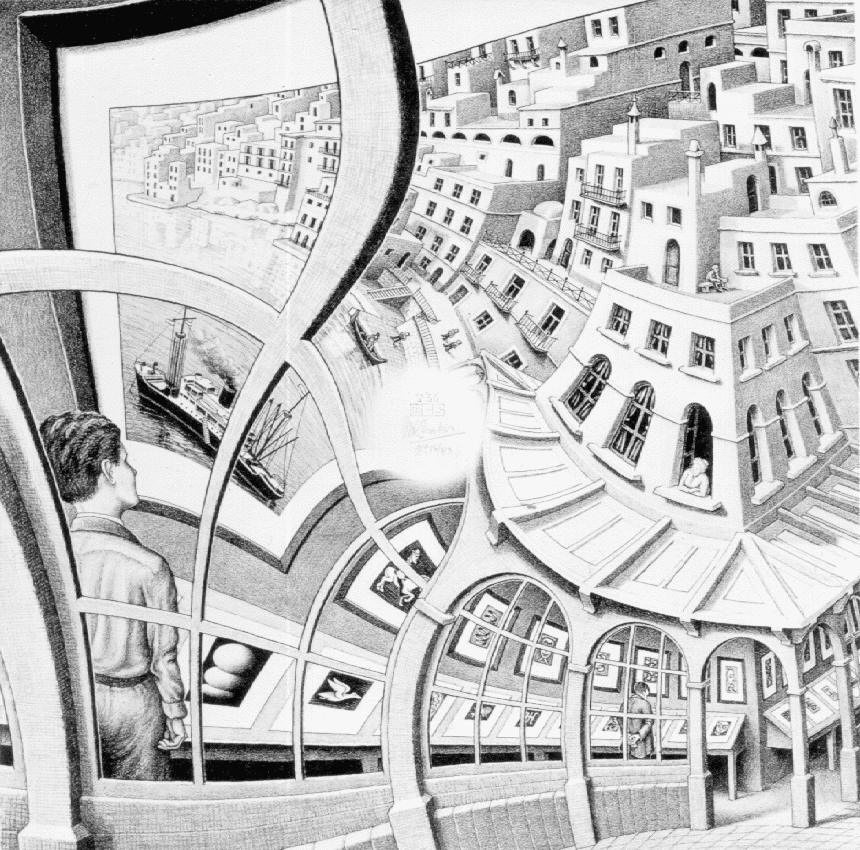
\includegraphics[width=0.5\columnwidth]{galleria_stampe} 
\caption[A floating figure]{A floating figure (the lithograph \emph{Galleria di stampe}, of M.~Escher, got from \url{http://www.mcescher.com/}).}
\label{fig:galleria} 
\end{figure}

\begin{figure}[tb] 
\centering 
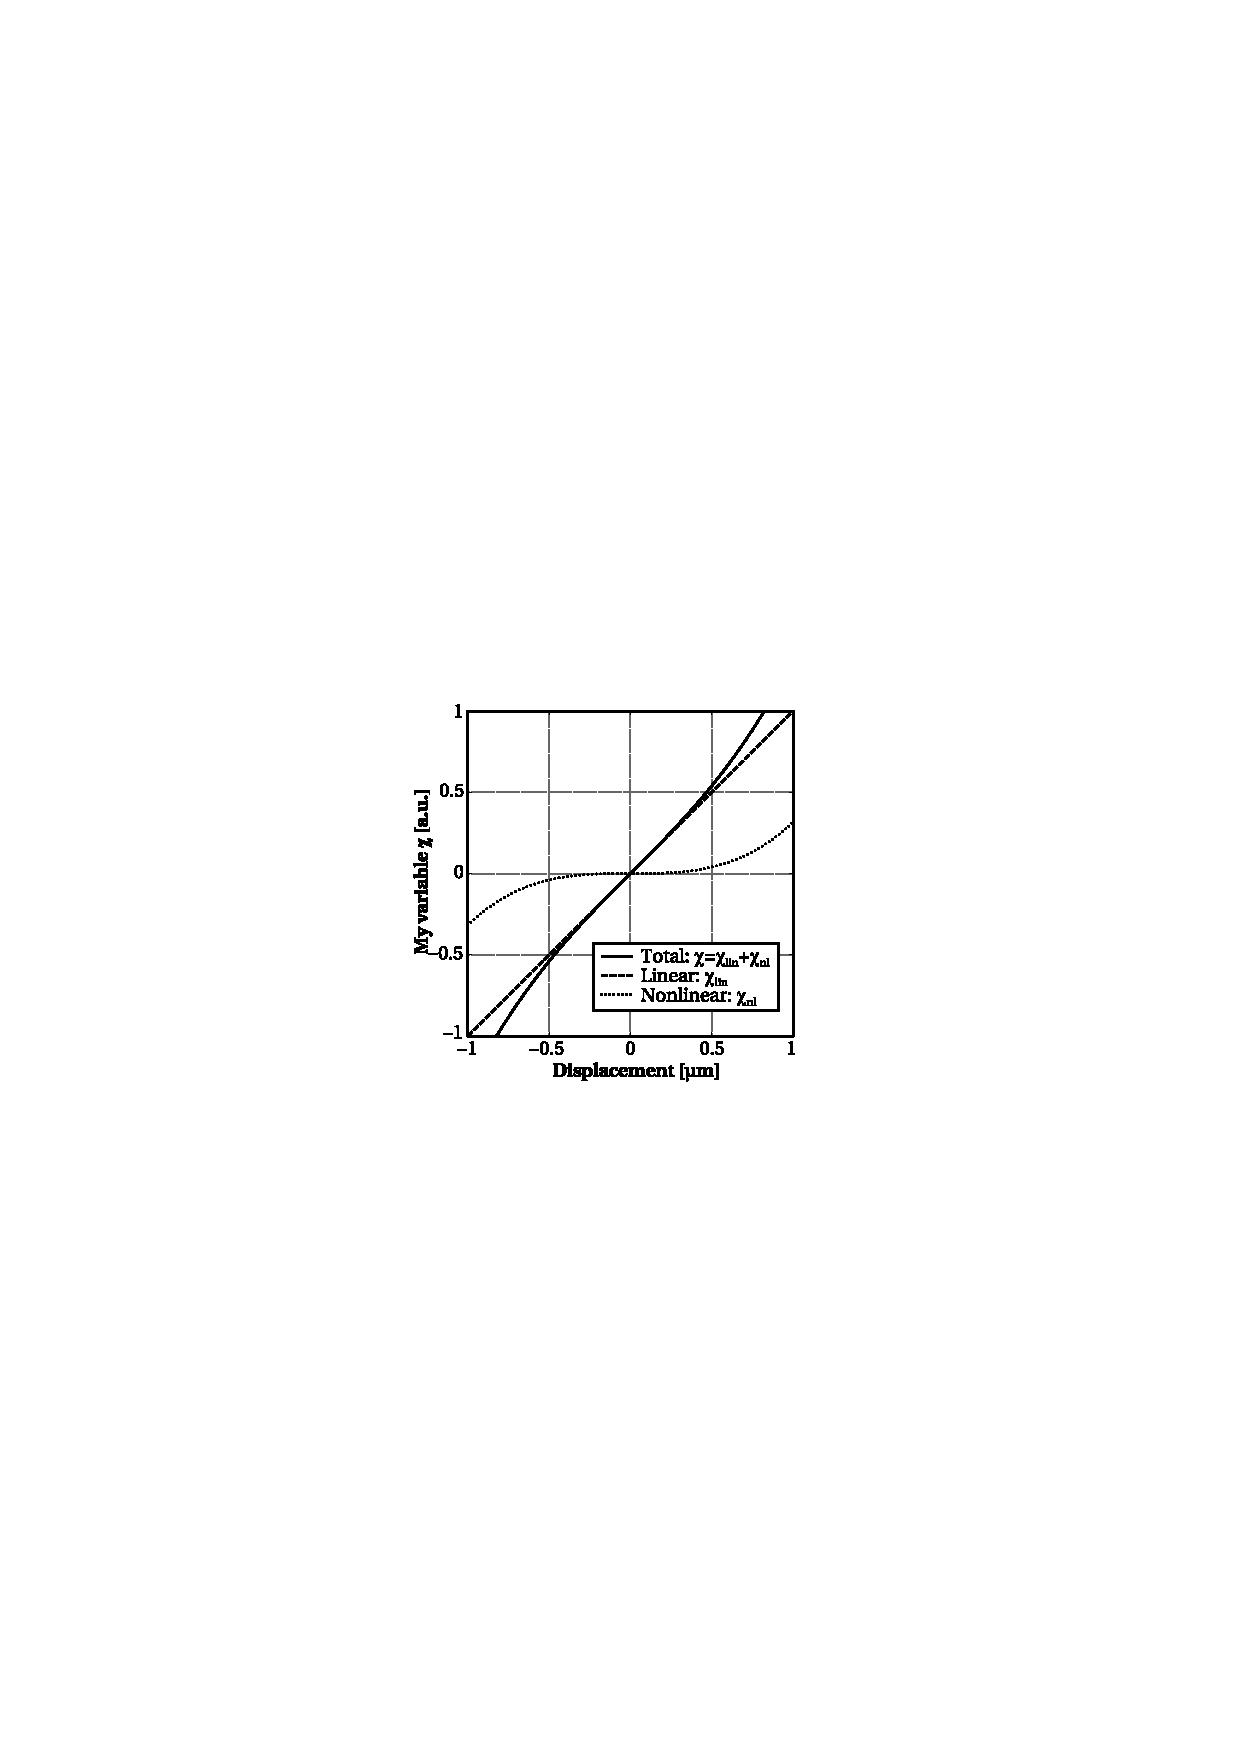
\includegraphics{some_vector_graphics.pdf} 
\caption[A floating figure]{A floating figure with text typeset in "Utopia Latex", a font provided in the template-folder for typesetting figures with greek characters. The text has been "outlined" for best compatibility with the repro during the printing.}
\label{fig:vector_graphics} 
\end{figure}


The figure~\ref{fig:galleria} is a floating figure and was obtained with the following code:
\begin{lstlisting}
\begin{figure}[tb] 
\centering 
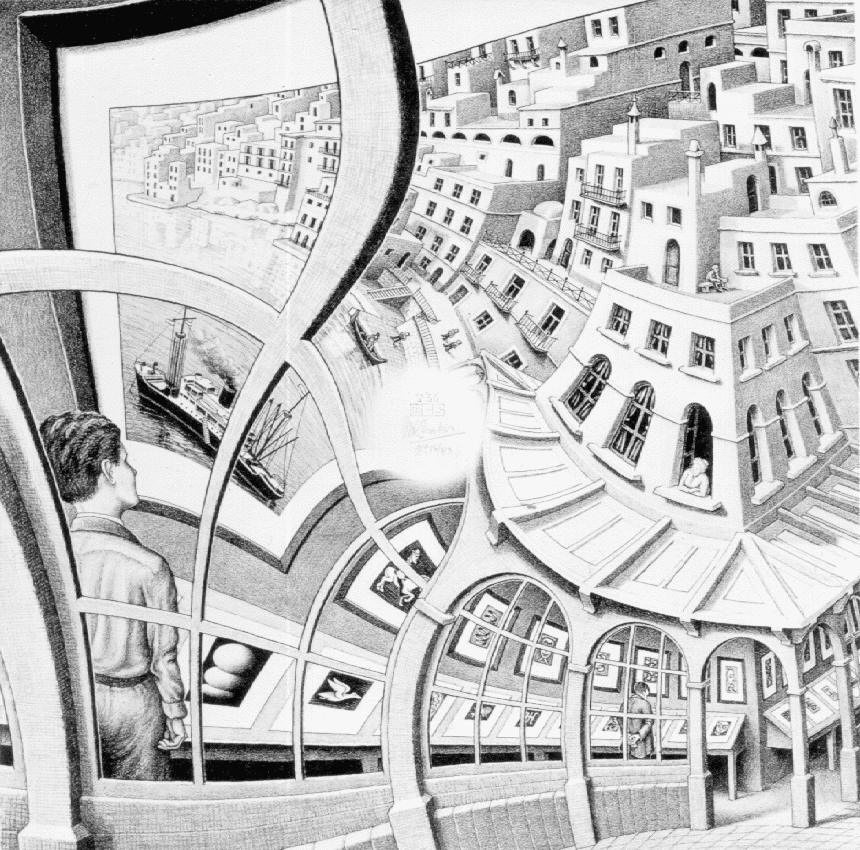
\includegraphics[width=0.5\columnwidth]{galleria_stampe} 
\caption[A floating figure]{A floating figure ... }
\label{fig:galleria} 
\end{figure}
\end{lstlisting}


\lipsum[1-2]

\begin{figure}[tb]
\centering

\subfloat[Asia personas duo.]
{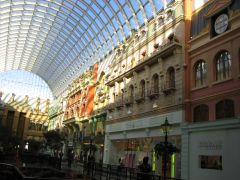
\includegraphics[width=.45\columnwidth]{lorem}} \quad
\subfloat[Pan ma signo.]
{\label{fig:ipsum}%
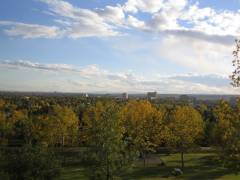
\includegraphics[width=.45\columnwidth]{ipsum}} \\
\subfloat[Methodicamente o uno.]
{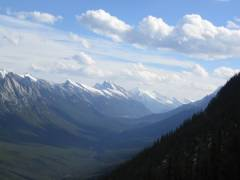
\includegraphics[width=.45\columnwidth]{dolor}} \quad
\subfloat[Titulo debitas.]
{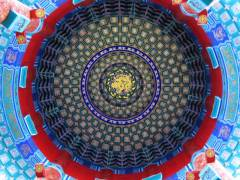
\includegraphics[width=.45\columnwidth]{sit}}
\caption[Tu duo titulo debitas latente]{Tu duo titulo debitas
latente.}
\label{fig:esempio}
\end{figure}

The figure~\ref{fig:esempio} is a floating figure and was obtained with the following code:
\begin{lstlisting}
\begin{figure}[tb]
\centering
\subfloat[Asia personas duo.]
{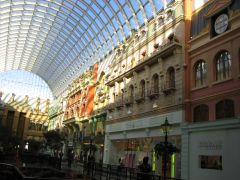
\includegraphics[width=.45\columnwidth]{lorem}} \quad
\subfloat[Pan ma signo.]
{\label{fig:ipsum}%
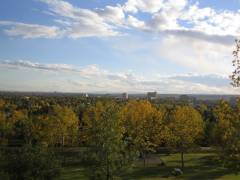
\includegraphics[width=.45\columnwidth]{ipsum}} \\
\subfloat[Methodicamente o uno.]
{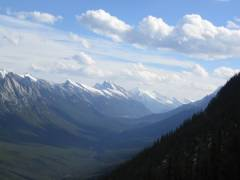
\includegraphics[width=.45\columnwidth]{dolor}} \quad
\subfloat[Titulo debitas.]
{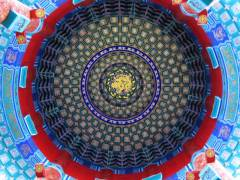
\includegraphics[width=.45\columnwidth]{sit}}
\caption[Tu duo titulo debitas latente]{Tu duo titulo debitas latente.}
\label{fig:esempio}
\end{figure}
\end{lstlisting}


\lipsum[3-8]

%\chapter{Mathematics}
In this chapter we will see some examples of mathematics.

\lipsum[1]

\section{Very important formulas}
\lipsum[2]

\begin{equation}\label{eqn:rate_eqns}
\frac{\textrm{d}}{\textrm{d}t}\left[
\begin{array}{l}
P_{\textit{0}} \\
P_{\textit{1}} \\
P_{\textit{T}}
\end{array}
\right] =
\left[
\begin{array}{l}
\frac{P_{\textit{1}}}{\tau_{\textit{10}}} + \frac{P_{\textit{T}}}{\tau_{\textit{T}}} - \frac{P_{\textit{0}}}{\tau_{\textit{ex}}} \\
- \frac{P_{\textit{1}}}{\tau_{\textit{10}}} - \frac{P_{\textit{1}}}{\tau_{isc}} + \frac{P_{\textit{0}}}{\tau_{\textit{ex}}} \\
\frac{P_{\textit{1}}}{\tau_{isc}} -  \frac{P_{\textit{T}}}{\tau_{\textit{T}}}
\end{array}
\right]
\end{equation}

\lipsum[3]


\begin{equation}\label{eqn:avgfluorescence}
\bar{I_{f}}(\vec{r})	 
	= \gamma(\vec{r}) \left(1 - \frac{\tau_{\textit{T}} P_{\textit{T}}^{{eq}}\left(1-\exp \left(-\frac{(T_p - t_p)}{\tau_{\textit{T}}}\right)\right)}{1-\exp\left(-\frac{(T_p - t_p)}{\tau_{\textit{T}}} + k_{\textit{2}} t_p\right)} \times \frac{\left(\exp\left(k_{\textit{2}} t_p\right)-1\right)}{t_p} \right) 
\end{equation}

\lipsum[3]

%\chapter{Another chapter}
Here you can see a citation: \cite{atc13}.

\lipsum[7]



%%%%%%%%%%%%%%%%%%%%%%%%%%%%%%%%%%%%%%%%%%%%%%
%%%%% TAIL: Bibliography, Appendix, CV
%%%%%%%%%%%%%%%%%%%%%%%%%%%%%%%%%%%%%%%%%%%%%%
%% Author :  Lionel du Peloux
% Contact : lionel.dupeloux@gmail
% Year : 2017

\newrefsegment
\chapter{Calculus of variations}\label{chp=variation}

% --------------------------------------------------------------------------------------------
\section{Introduction}
% --------------------------------------------------------------------------------------------
In this appendix we drawback essential mathematical concepts for the calculus of variations \cite{Abraham2002}.
Recall how the notion of energy, gradients are extended to function spaces.


% --------------------------------------------------------------------------------------------
\section{Spaces}
% --------------------------------------------------------------------------------------------

\subsection{Normed space}
% --------------------------------------------------------------------------------------------
A \emph{normed space} $V(\mathbb{K})$ is a vector space $V$ over the scalar field $\mathbb{K}$ with a norm $\|.\|$.

A \emph{norm} is a map $\| . \|~: V \times V \longmapsto \mathbb{K}$ which satisfies~:
\begin{subequations}
\begin{align}
	&\forall x \in V, 							&& \|x\| = 0_\mathbb{K} \Rightarrow x = 0_V&&&\\
	&\forall x \in V, \forall \lambda \in \mathbb{K}, 	&& \|\lambda x\| = |\lambda| \,\|x\|&&&\\
	&\forall (x,y) \in V^2, 						&& \|x + y\| \leqslant \|x\| + \|y\|&&&
\end{align}
\end{subequations}


\subsection{Inner product space}
% --------------------------------------------------------------------------------------------
A \emph{inner product space} or \emph{pre-hilbert space} $E(\mathbb{K})$ is a vector space $E$ over the scalar field $\mathbb{K}$ with an inner product.

An \emph{inner product} is a map $\langle \,; \rangle~: E \times E \longmapsto \mathbb{K}$ which is bilinear, symmetric and positive-definite~:
\begin{subequations}
\begin{align}
	&\forall (x,y,z) \in E^3, \forall (\lambda,\mu) \in \mathbb{K}^2, 	&& \langle \lambda x\ + \mu y \,; z\rangle  = \lambda \langle  x \,; z\rangle + \mu \langle  y\,; z\rangle&&&\\
	&												&& \langle x \,; \lambda y + \mu z \rangle  = \lambda \langle  x\,; y\rangle + \mu \langle  x \,; z\rangle&&&\notag\\
	&\forall (x,y) \in E^2, 									&& \langle x\,; y\rangle = \langle y\,; x\rangle &&&\\
	&\forall x \in E, 										&& \langle x\,; x\rangle \geqslant 0_\mathbb{K} &&&\\
	&\forall x \in E, 										&& \langle x\,; x\rangle = 0_\mathbb{K} \Rightarrow x = 0_E &&&
\end{align}
\end{subequations}
Moreover, an inner product naturally induces a norm on $E$ defined by~:
\begin{align}
	\forall x \in E, \quad \|x\| = \sqrt{\langle x\,; x\rangle}
\end{align}
Thus, an inner product vector space is also naturally a normed vector space.

\subsection{Euclidean space}
% --------------------------------------------------------------------------------------------
An \emph{Euclidean space} $\mathcal{E}(\mathbb{R})$ is a finite-dimensional real vector space with an inner product.
Thus, distances and angles between vectors could be defined and measured regarding to the norm associated with the chosen inner product.

An Euclidean space is nothing but a finite-dimensional real pre-hilbert space.

\subsection{Banach space}
% --------------------------------------------------------------------------------------------

A \emph{Banach space} $\mathcal{B}(\mathbb{K})$ is a complete normed vector space, which means that it is a normed vector space in which every Cauchy sequence of $\mathcal{B}$ converges in $\mathcal{B}$ for the given norm.

Thus, a Banach space is a vector space with a metric that allows the computation of vector length and distance between vectors and is complete in the sense that a Cauchy sequence of vectors always converges to a well defined limit in that space.

\subsection{Hilbert space}
% --------------------------------------------------------------------------------------------

A \emph{Hilbert space} is an inner product vector space $\mathcal{H}(\mathbb{K})$ such that the natural norm induced by the inner product turns $\mathcal{H}$ into a complete metric space (i.e.\ every Cauchy sequence of $\mathcal{H}$ converges in $\mathcal{H}$).

The Hilbert space concept is a generalization of the Euclidean space concept.
In physics it's common to encounter Hilbert spaces as infinite-dimensional function spaces.

Hilbert spaces are Banach spaces, but the converse does not hold generally.

For example, $\mathcal{L}^2([a,b])$ is an infinite-dimensional Hilbert space with the canonical inner product $\langle f\,; g\rangle=\int_a^b fg$.

Note that $\mathcal{L}^2$ is the only Hilbert space among the $\mathcal{L}^p$ spaces.
% --------------------------------------------------------------------------------------------
\section{Derivative}
% --------------------------------------------------------------------------------------------

The well known notion of function derivative in $\mathbb{R}^\mathbb{R}$ can be extended to maps between Banach spaces.
This is useful in physics when formulating problems as variational problems, usually in terms of energy minimization. Indeed, energy is generally defined over a functional vector space and not simply over the real line.

In this case, the research of minimal values of a potential energy rests on the calculus of variations of the energy function compared to variations to other functions defining the problem (geometry, materials, boundary conditions, ...).

Mathematical concepts extended well-known notions of derivative, jacobian and hessian in Euclidean spaces (typically $\mathbb{R}^2$ or $\mathbb{R}^3$) for Banach functional spaces.

\subsection{Fréchet derivative}
% --------------------------------------------------------------------------------------------
\subsubsection{Differentiability}
Let $\mathcal{B}_V$ and $\mathcal{B}_W$ be two Banach spaces and $U \subset \mathcal{B}_V$ an open subset of $\mathcal{B}_V$.
Let $\fonction{f}{u}{f(u)}$ be a function of  $U^{\mathcal{B}_W}$.
$f$ is said to be \emph{Fréchet differentiable} at $u_0\in U$ if there exists a continious linear operator $\diff{f}{u_0} \in
\mathcal{L}(\mathcal{B}_V,{\mathcal{B}_W})$ such that~:
\begin{subequations}
\begin{align}
\lim_{h \to 0} \frac{f(u_0+h) - f(u_0)- \diffof{f}{u_0}{h}}{\|h\|} = 0
\end{align}
\text{Or, equivalently~:}
\begin{align}
	f(u_0+h) = f(u_0) + \diffof{f}{u_0}{h} + o(h) \quad , \quad
	\lim_{h \to 0} \frac{o(h)}{\|h\|} = 0
\end{align}
\end{subequations}

In the literature, it is common to found the following notations~: $df = \diffof{f}{u_0}{h} = \boldsymbol{D}f_{u_0}(h) = \boldsymbol{D}f(u_0,h)$ for the differential of $f$, which means nothing but $\boldsymbol{D}f(u_0)$ is linear regarding $h$. The dot denotes the evaluation of $\boldsymbol{D}f(u_0)$ at $h$. This notation can be ambiguous as far as the linearity of $\boldsymbol{D}f(u_0)$ in $h$ is denoted as a product which is not explicitly defined.

\subsubsection{Derivative}

If $f$ is Fréchet differentiable at $u_0 \in U$, the continous linear operator $\diff{f}{u_0} \in
\mathcal{L}(\mathcal{B}_V,{\mathcal{B}_W})$ is called the \emph{Fréchet derivative} of $f$ at $u_0$ and is also denoted~:
\begin{align}
	f'(u_0) = \diff{f}{u_0}
\end{align}
$f$ is said to be $\mathcal{C}^1$ in the sens of Fréchet if $f$ is Fréchet differentiable for all $u \in U$ and the function $\fonction{\boldsymbol{D}f}{u}{f'(u)}$ of $U^{\mathcal{L}(\mathcal{B}_V,{\mathcal{B}_W})}$ is continuous.

\subsubsection{Differential or total derivative}

$df = \diffof{f}{u_0}{h}$ is sometimes called the \emph{differential} or \emph{total derivative} of $f$ and represents the change in the function $f$ for a perturbation $h$ from $u_0$.

\subsubsection{Higer derivatives}

Because the differential of $f$ is a linear map from $\mathcal{B}_V$ to $\mathcal{L}(\mathcal{B}_V,{\mathcal{B}_W})$ it is possible to look for the differentiability of $\boldsymbol{D}f$. If it exists, it is denoted $\boldsymbol{D}^2f$ and maps $\mathcal{B}_V$ to $\mathcal{L}(\mathcal{B}_V,\mathcal{L}(\mathcal{B}_V,{\mathcal{B}_W}))$.

\subsection{Gâteaux derivative}
% --------------------------------------------------------------------------------------------
\subsubsection{Directional derivative}
Let $\mathcal{B}_V$ and $\mathcal{B}_W$ be two Banach spaces and $U \subset \mathcal{B}_V$ an open subset of $\mathcal{B}_V$.
Let $\fonction{f}{u}{f(u)}$ be a function of  $U^{\mathcal{B}_W}$.
$f$ is said to have a \emph{derivative in the direction} $h\in\mathcal{B}_V$ at $u_0\in U$ if~:
\begin{align}
\frac{d}{d\lambda}f(u_0+\lambda h)\Bigr|_{\lambda = 0} = \lim_{\lambda \to 0} \frac{f(u_0+\lambda h) - f(u_0)}{\lambda}
\end{align}
exists. This element of $\mathcal{B}_W$ is called the \emph{directional derivative} of $f$ in the direction $h$ at $u_0$.

\subsubsection{Differentiability}
Let $\mathcal{B}_V$ and $\mathcal{B}_W$ be two Banach spaces and $U \subset \mathcal{B}_V$ an open subset of $\mathcal{B}_V$.
Let $\fonction{f}{u}{f(u)}$ be a function of  $U^{\mathcal{B}_W}$.
$f$ is said to be \emph{Gâteaux differentiable} at $u_0\in U$ if there exists a continious linear operator $\diff{f}{u_0} \in
\mathcal{L}(\mathcal{B}_V,{\mathcal{B}_W})$ such that~:
\begin{subequations}
\begin{align}
\forall h \in \mathcal{U}, \quad\lim_{\lambda \to 0} \frac{f(u_0+\lambda h) - f(u_0)}{\lambda} = \frac{d}{d\lambda}f(u_0+\lambda h)\Bigr|_{\lambda = 0} = \diffof{f}{u_0}{h}
\end{align}
Or, equivalently~:
\begin{align}
	\forall h \in \mathcal{U}, \quad f(u+\lambda h) = f(u) + \lambda \diffof{f}{u_0}{h} + o(\lambda)
	\quad , \quad \lim_{\lambda \to 0} \frac{o(\lambda)}{\lambda} = 0
\end{align}
\end{subequations}

In other words, it means that all the directional derivatives of $f$ exist at $u_0$.

\subsubsection{Derivative}
If $f$ is Gâteaux differentiable at $u_0 \in U$, the continous linear operator $\diff{f}{u_0} \in
\mathcal{L}(\mathcal{B}_V,{\mathcal{B}_W})$ is called the \emph{Gâteaux derivative} of $f$ at $u_0$ and is also denoted~:
\begin{align}
	f'(u_0) = \diff{f}{u_0}
\end{align}
$f$ is said to be $\mathcal{C}^1$ in the sens of Gâteaux if $f$ is Gâteaux differentiable for all $u \in U$ and the function $\fonction{\boldsymbol{D}f}{u}{f'(u)}$ of $U^{\mathcal{L}(\mathcal{B}_V,{\mathcal{B}_W})}$ is continuous.

The Gâteaux derivative is a weaker form of derivative than the Fréchet derivative. If $f$ is Fréchet differentiable, then it is also Gâteaux differentiable and its Fréchet and Gâteaux derivatives agree, but the converse does not hold generally.

\subsection{Useful properties}

Let $\mathcal{B}_V$, $\mathcal{B}_W$ and $\mathcal{B}_Z$ be three Banach spaces.
Let $f,g~: \mathcal{B}_V \longmapsto \mathcal{B}_W$ and $h~: \mathcal{B}_W \longmapsto \mathcal{B}_Z$ be three Gâteaux differentiable functions. Then, the following useful properties holds~:
\begin{align}
	&\diff{(f+g)}{u} = \diff{f}{u} + \diff{g}{u}\\
	&\diff{(f \circ h)}{u} = \diff{h}{f(u)}\circ\diff{f}{u} = \diff{h}{f(u)}\cdot\diff{f}{u}
\end{align}
Recall that the composition of $\diff{h}{f(u)}$ with $\diff{f}{u}$ means \textquote{$\diff{h}{f(u)}$ applied to $\diff{f}{u}$} and is also denoted by $\cdot$ as explained previously.

\subsection{Partial derivative}

Following~\cite{Abraham2002} the main results on partial derivatives of two-variables functions are presented here. They are generalizable to n-variables functions.

\subsubsection{Definition}

Let $\mathcal{B}_{V_1}$, $\mathcal{B}_{V_2}$ and $\mathcal{B}_W$ be three Banach spaces and $U \subset \mathcal{B}_{V_1}\oplus\mathcal{B}_{V_2}$ an open subset of $\mathcal{B}_{V_1}\oplus\mathcal{B}_{V_2}$.
Let $\fonction{f}{u}{f(u)}$ be a function of  $U^{\mathcal{B}_W}$.
Let $u_0 = (u_{01},u_{02}) \in U$.
If the derivatives of the following functions exist~:
\begin{equation}
	\fonctionL{f_1}{\mathcal{B}_{V_1}}{\mathcal{B}_{W}}{u_1}{f(u_1,u_{02})}
	\quad , \quad
	\fonctionL{f_2}{\mathcal{B}_{V_2}}{\mathcal{B}_{W}}{u_2}{f(u_{01},u_{2})}
\end{equation}
they are called \emph{partial derivatives} of $f$ at $u_0$ and are denoted $\pdiff{1}{f}{u_0} \in
\mathcal{L}(\mathcal{B}_{V_1},{\mathcal{B}_W})$ and $\pdiff{2}{f}{u_0} \in
\mathcal{L}(\mathcal{B}_{V_2},{\mathcal{B}_W})$.

\subsubsection{Differentiability}

Let $\mathcal{B}_{V_1}$, $\mathcal{B}_{V_2}$ and $\mathcal{B}_W$ be three Banach spaces and $U \subset \mathcal{B}_{V_1}\oplus\mathcal{B}_{V_2}$ an open subset of $\mathcal{B}_{V_1}\oplus\mathcal{B}_{V_2}$.
Let $\fonction{f}{u}{f(u)}$ be a function of  $U^{\mathcal{B}_W}$.
If $f$ is differentiable, then the partial derivatives exist and satisfy for all $h = (h_1,h_2) \in \mathcal{B}_{V_1}\oplus\mathcal{B}_{V_2}$~:
\begin{align}
	&\pdiffof{1}{f}{u}{h_1} = \diffof{f}{u}{(h_1,0)} \\
	&\pdiffof{2}{f}{u}{h_2} = \diffof{f}{u}{(0,h_2)} \\
	&\diffof{f}{u}{(h_1,h_2)} = \pdiffof{1}{f}{u}{h_1} + \pdiffof{2}{f}{u}{h_2}
\end{align}

\section{Gradient vector}

Let $\mathcal{H}$ be a Hilbert space with the inner product denoted $\scalar{}{}$. Let $U \subset \mathcal{H}$ an open subset of $\mathcal{H}$.
Let $\fonction{F}{u}{F(u)}$ be a scalar function of  $U^{\mathbb{R}}$.
The \emph{gradient} of $F$ is the map $\fonction{\grad{F}}{x}{(\grad{F})(x)}$ of $U^{\mathcal{H}}$ such that~:
\begin{equation}
	\forall h \in \mathcal{H}, \quad  \scalar{(\grad{F})(x)}{h} = \diffof{F}{x}{h}
\end{equation}
Note that the gradient vector depends on the chosen inner product.
For $\mathcal{H} = \mathbb{R}^{n}$ with the canonical inner product, one can recall the usual definition of the gradient vector and the corresponding linear approximation of $F$~:
\begin{equation}
	\mat{F}_{x+h} = \mat{F}_{x} + (\grad{F})_{x}^T H + \mat{o}(H)
	\quad , \quad \grad{F}_{x} = \left[\begin{array}{c}\frac{\partial F}{\partial x_1} \\ \vdots \\ \frac{\partial F}{\partial x_n}\end{array}\right] \in \mathbb{R}^n
\end{equation}
Recall that the canonical inner product on $\mathbb{R}^{n}$ is such that $\scalar{x}{y} = X^{T}Y$ in a column vector representation. In this case it is common to denote $\grad{F} = \nabla{F}$.

For function spaces the usual definition of the gradient can be extended. For instance if $F$ is a scalar function on $\mathcal{L}^2$, the gradient of $F$ is the unique function (if it exists) from $\mathcal{L}^2$ which satisfies~:
\begin{equation}
	\forall h \in \mathcal{L}^2, \quad \diffof{F}{x}{h} = \scalar{(\grad{F})(x)}{h} = \int (\grad{F})h
\end{equation}
In this case it is common to denote $\grad{F} = \frac{\delta F}{\delta x}$. The gradient is also known as the \emph{functional derivative}. The existence and unicity of $\grad{F}$ is ensured by the \emph{Riesz representation theorem}.

\section{Jacobian matrix}
Let $f$ be a differentiable function from $\mathbb{R}^n$ to $\mathbb{R}^m$. The \emph{differential} or \emph{total derivative} of such a fonction is a linear application from $\mathbb{R}^n$ to $\mathbb{R}^m$ which could be represented with the following matrix called the \emph{jacobian matrix}~:
\begin{align}
	&\diff{f}{x} = \mat{J}_x = \frac{df}{dx} =
	\begin{bmatrix}
		\frac{\partial f}{\partial x_1}&\cdots&\frac{\partial f}{\partial x_n}
	\end{bmatrix}=
	\begin{bmatrix}
		\frac{\partial f_1}{\partial x_1} & \cdots & \frac{\partial f_1}{\partial x_n} \\
		\vdots & \ddots & \vdots \\
		\frac{\partial f_m}{\partial x_1} & \cdots & \frac{\partial f_m}{\partial x_n}
	\end{bmatrix}
	\in\mathcal{M}_{m,n}(\mathbb{R})
\end{align}
Thus, with the matrix notation, the Taylor expansion takes the following form~:
\begin{align}
	&\mat{F}_{x+h} = \mat{F}_{x} +  \boldsymbol{J}_x H + \mat{o}(H)
\end{align}
In the cas $m=1$, the jacobian matrix of the functional $F$ is nothing but the gradient vector transpose itself~:
\begin{align}
	\diff{F}{x} = \mat{J}_x = \frac{dF}{dx} =
	\begin{bmatrix}
		\frac{\partial F}{\partial x_1}& \cdots&\frac{\partial F}{\partial x_n}
	\end{bmatrix} = \nabla F^T
\end{align}

\section{Hessian}
Let $F$ be a differentiable scalar function from $\mathbb{R}^n$ to $\mathbb{R}$. The second order differential of such a fonction is a linear application from $\mathbb{R}^n$ to $\mathbb{R}^n$ which could be represented with the following matrix called the \emph{hessian matrix}~:
\begin{equation}
\renewcommand\arraystretch{1.5}
\begin{aligned}
	&\boldsymbol{D}^{2}F(x) = \mat{H}_{x} = \frac{d^2F}{dx}(x) =
	\begin{bmatrix}
		\frac{\partial^2 F}{\partial x_1^2} & \frac{\partial^2 F}{\partial x_1\partial x_2} &\cdots & \frac{\partial^2 F}{\partial x_1\partial x_n} \\
		\frac{\partial^2 F}{\partial x_2\partial x_1} & \frac{\partial^2 F}{\partial x_2^2} &\cdots & \frac{\partial^2 F}{\partial x_2\partial x_n} \\
		\vdots & &\ddots & \vdots \\
		\frac{\partial^2 F}{\partial x_n\partial x_1} & \frac{\partial^2 F}{\partial x_n\partial x_2}&\cdots & \frac{\partial^2 F}{\partial x_n^2}
	\end{bmatrix}
	\in\mathcal{M}_{n,n}(\mathbb{R})
\end{aligned}
\end{equation}
Thus, with the matrix notation, the Taylor expansion takes the following form~:
\begin{align}
	\mat{F}_{x+h} = \mat{F}_{x} +  \mat{J}_{x} H + \tfrac{1}{2}H^T \mat{H}_{x} H + \mat{o}(H)
\end{align}


\section{Functional}
% --------------------------------------------------------------------------------------------
A \emph{functional} is a map from a vector space $E(\mathbb{K})$ into its underlying scalar field $\mathbb{K}$. Here $\mathcal{E}_p[\boldsymbol{x},\theta]$ is a functional depending over $\boldsymbol{x}$ and $\theta$.
%\appendix
\chapter{Calculus of variations}

% --------------------------------------------------------------------------------------------
\section{Introduction}
% --------------------------------------------------------------------------------------------
In this appendix we drawback essential mathematical concepts for the calculus of variations.
Recall how the notion of energy, gradients are extended to function spaces.

\cite{Abraham2002}

% --------------------------------------------------------------------------------------------
\section{Spaces}
% --------------------------------------------------------------------------------------------

\subsection{Normed space}
% --------------------------------------------------------------------------------------------
A \emph{normed space} $V(\mathbb{K})$ is a vector space $V$ over the scalar field $\mathbb{K}$ with a norm $\|.\|$.

A \emph{norm} is a map $\| . \| : V \times V \longmapsto \mathbb{K}$ which satisfies :
\begin{align}
	&\forall x \in V, 							&& \|x\| = 0_\mathbb{K} \Rightarrow x = 0_V&&&\\
	&\forall x \in V, \forall \lambda \in \mathbb{K}, 	&& \|\lambda x\| = |\lambda| \,\|x\|&&&\\
	&\forall (x,y) \in V^2, 						&& \|x + y\| \leqslant \|x\| + \|y\|&&&
\end{align}

\subsection{Inner product space}
% --------------------------------------------------------------------------------------------
A \emph{inner product space} or \emph{pre-hilbert space} $E(\mathbb{K})$ is a vector space $E$ over the scalar field $\mathbb{K}$ with an inner product.

An \emph{inner product} is a map $\langle \,; \rangle : E \times E \longmapsto \mathbb{K}$ which is bilinear, symmetric, positive-definite :
\begin{align}
	&\forall (x,y,z) \in E^3, \forall (\lambda,\mu) \in \mathbb{K}^2, 	&& \langle \lambda x\ + \mu y \,; z\rangle  = \lambda \langle  x \,; z\rangle + \mu \langle  y\,; z\rangle&&&\\
	&												&& \langle x \,; \lambda y + \mu z \rangle  = \lambda \langle  x\,; y\rangle + \mu \langle  x \,; z\rangle&&&\notag\\
	&\forall (x,y) \in E^2, 									&& \langle x\,; y\rangle = \langle y\,; x\rangle &&&\\
	&\forall x \in E, 										&& \langle x\,; x\rangle \geqslant 0_\mathbb{K} &&&\\
	&\forall x \in E, 										&& \langle x\,; x\rangle = 0_\mathbb{K} \Rightarrow x = 0_E &&&
\end{align}
Moreover, an inner product naturally induces a norm on $E$ defined by :
\begin{align}
	\forall x \in E, \quad \|x\| = \sqrt{\langle x\,; x\rangle}
\end{align}
Thus, an inner product vector space is also naturally a normed vector space.

\subsection{Euclidean space}
% --------------------------------------------------------------------------------------------
An \emph{Euclidean space} $\mathcal{E}(\mathbb{R})$ is a finite-dimensional real vector space with an inner product.
Thus, distances and angles between vectors could be defined and measured regarding to the norm associated with the chosen inner product.

An Euclidean space is nothing but a finite-dimensional real pre-hilbert space.

\subsection{Banach space}
% --------------------------------------------------------------------------------------------

A \emph{Banach space} $\mathcal{B}(\mathbb{K})$ is a complete normed vector space, which means that it is a normed vector space in which every Cauchy sequence of $\mathcal{B}$ converges in $\mathcal{B}$ for the given norm.

Thus, a Banach space is a vector space with a metric that allows the computation of vector length and distance between vectors and is complete in the sense that a Cauchy sequence of vectors always converges to a well defined limit in that space.

\subsection{Hilbert space}
% --------------------------------------------------------------------------------------------

A \emph{Hilbert space} is an inner product vector space $\mathcal{H}(\mathbb{K})$ such that the natural norm induced by the inner product turns $\mathcal{H}$ into a complete metric space (i.e.\ every Cauchy sequence of $\mathcal{H}$ converges in $\mathcal{H}$).

The Hilbert space concept is a generalization of the Euclidean space concept.
In physics it's common to encounter Hilbert spaces as infinite-dimensional function spaces.

Hilbert spaces are Banach spaces, but the converse does not hold generally.

For example, $\mathcal{L}^2([a,b])$ is an infinite-dimensional Hilbert space with the canonical inner product $\langle f\,; g\rangle=\int_a^b fg$.

Note that $\mathcal{L}^2$ is the only Hilbert space among the $\mathcal{L}^p$ spaces.
% --------------------------------------------------------------------------------------------
\section{Derivative}
% --------------------------------------------------------------------------------------------

The well known notion of function derivative in $\mathbb{R}^\mathbb{R}$ can be extended to maps between Banach spaces.
This is useful in physics when formulating problems as variational problems, usually in terms of energy minimization. Indeed, energy is generally defined over a functional vector space and not simply over the real line.

In this case, the research of minimal values of a potential energy rests on the calculus of variations of the energy function compared to variations to other functions defining the problem (geometry, materials, boundary conditions, ...).

Mathematical concepts extended well-known notions of derivative, jacobian and hessian in Euclidean spaces (typically $\mathbb{R}^2$ or $\mathbb{R}^3$) for Banach functional spaces.

\subsection{Fréchet derivative - strong}
% --------------------------------------------------------------------------------------------
\subsubsection{Differentiability}
Let $\mathcal{B}_V$ and $\mathcal{B}_W$ be two Banach spaces and $U \subset \mathcal{B}_V$ an open subset of $\mathcal{B}_V$.
Let $f : u \longmapsto f(u)$ be a function of  $U^{\mathcal{B}_W}$.
$f$ is said to be \emph{Fréchet differentiable} at $u\in U$ if there exists a continious linear operator $Df_{u} \in 
\mathcal{L}(\mathcal{B}_V,{\mathcal{B}_W})$ such that :
\begin{align}
\lim_{\|h\| \to 0} \frac{\|f(u+h) - f(u)- Df_{u}(h)\|_{\mathcal{B}_W}}{\|h\|_{\mathcal{B}_V}} = 0
\end{align}
Or, equivalently :
\begin{align}
	f(u+h) = f(u) + Df_{u}(h) + o(\|h\|) \quad , \quad 
	\lim_{\|h\| \to 0} \frac{\|o(\|h\|)\|_{\mathcal{B}_W}}{\|h\|} = 0
\end{align}

Note that $df = Df_{u}(h)$ is called the differential of $f$ at point $u$ and represents the change in the function $f$ for a perturbation $h$ from $u$.

In the literature, it is common to found the following notation : $df = Df_u(h) = Df(u)h$, for the differential of $f$, which means nothing but $Df(u)$ is linear regarding $h$. This notation can be ambiguous as far as the linearity of $Df(u)$ in $h$ is denoted as a product which is not explicitly defined.

\subsubsection{Derivability}

If $f$ is Fréchet differentiable at $u \in U$, the continous linear operator $Df_{u} \in 
\mathcal{L}(\mathcal{B}_V,{\mathcal{B}_W})$ is called the Fréchet derivative of $f$ at $u$ and is also denoted :
\begin{align}
	f'(u) = Df(u) = Df_{u}
\end{align}
$f$ is said to be $\mathcal{C}^1$ in the sens of Fréchet if $f$ is Fréchet differentiable for all $u \in U$ and the function $Df : u \longmapsto f'(u)$ of $U^{\mathcal{L}(\mathcal{B}_V,{\mathcal{B}_W})}$ is continuous.
 
\subsubsection{Higer derivatives}
 
Because the differential of $f$ is a linear map from $\mathcal{B}_V$ to $\mathcal{L}(\mathcal{B}_V,{\mathcal{B}_W})$ it is possible to look for the differentiability of $Df$. If it exists, it is denoted $D^2f$ and maps $\mathcal{B}_V$ to $\mathcal{L}(\mathcal{B}_V,\mathcal{L}(\mathcal{B}_V,{\mathcal{B}_W}))$.
 
\subsection{Gâteaux derivative - weak}
% --------------------------------------------------------------------------------------------
\subsubsection{Differentiability}
Let $\mathcal{B}_V$ and $\mathcal{B}_W$ be two Banach spaces and $U \subset \mathcal{B}_V$ an open subset of $\mathcal{B}_V$.
Let $f : u \longmapsto f(u)$ be a function of  $U^{\mathcal{B}_W}$.
$f$ is said to be \emph{Gâteaux differentiable} at $u\in U$ if there exists a continious linear operator $Df_{u} \in 
\mathcal{L}(\mathcal{B}_V,{\mathcal{B}_W})$ such that :
\begin{align}
\forall h \in \mathcal{U}, \quad\lim_{\lambda \to 0} \frac{f(u+\lambda h) - f(u)}{\lambda} = \frac{d}{d\lambda}f(u+\lambda h)\Bigr|_{\lambda = 0} = Df_u(h)
\end{align}
Or, equivalently :
\begin{align}
	\forall h \in \mathcal{U}, \quad f(u+\lambda h) = f(u) + \lambda D_{f,u}(h) + o(|\lambda|)
	\quad , \quad \lim_{\lambda \to 0} \frac{\|o(|\lambda|)\|_{\mathcal{B}_W}}{\lambda} = 0
\end{align}

Note that $df = Df_{u}(h)$ is called the differential of $f$ at point $u$.

\subsubsection{Derivability}
If $f$ is Gâteaux differentiable at $u \in U$, the continous linear operator $Df_{u} \in 
\mathcal{L}(\mathcal{B}_V,{\mathcal{B}_W})$ is called the Gâteaux derivative of $f$ at $u$ and is also denoted :
\begin{align}
	f'(u) = Df(u) = Df_{u}
\end{align}
$f$ is said to be $\mathcal{C}^1$ in the sens of Gâteaux if $f$ is Gâteaux differentiable for all $u \in U$ and the function $Df : u \longmapsto f'(u)$ of $U^{\mathcal{L}(\mathcal{B}_V,{\mathcal{B}_W})}$ is continuous.
 
The Gâteaux derivative is a weaker form of derivative than the Fréchet derivative : if $f$ is Fréchet differentiable, then it is also Gâteaux differentiable, and its Fréchet and Gâteaux derivatives agree, but the converse does not hold generally.

\subsection{Useful properties}

Let $\mathcal{B}_V$, $\mathcal{B}_W$ and $\mathcal{B}_Z$ be three Banach spaces. 
Let $f,g : \mathcal{B}_V \longmapsto \mathcal{B}_W$ and $h : \mathcal{B}_W \longmapsto \mathcal{B}_Z$ be three Gâteaux differentiable functions. Then, the following useful properties holds :
\begin{align}
	&D(f+g)(u) = Df(u) + Dg(u)\\
	&D(h\circ f)(u) = Dh(f(u)) \circ Df(u)
\end{align}

\subsection{Partial derivative}

\section{Gradient}

The \emph{gradient vector} denotes the differential or total derivative of a differentiable function $F$ in the special case it is a map from $\mathbb{R}^n$ to $\mathbb{R}$. Thus, it satisfies the following relationships :
\begin{align}
	&\nabla F(x) = F'(x) = DF_x\\
	&DF_x(h) = \langle \nabla F(x)\,; h\rangle\\
	&F(x + h) = F(x) + \langle \nabla F(x)\,; h\rangle + o(\|h\|)
\end{align}
If the matrix notation is adopted, the previous relations leads to :
\begin{align}
	{F}({X}+{H}) = F(X) +  \nabla F(u)^T H + o(\|H\|)
	\quad , \quad \nabla F(x) = \left[\begin{array}{c}\frac{\partial F}{\partial x_1} \\ \vdots \\ \frac{\partial F}{\partial x_n}\end{array}\right] \in \mathbb(R)^n
\end{align}

\section{Jacobian}
Let $f$ be a differentiable function from $\mathbb{R}^n$ to $\mathbb{R}^p$. The differential of such a fonction is a linear application from $\mathbb{R}^n$ to $\mathbb{R}^p$ which could be represented with the following matrix called the \emph{jacobian matrix} :
\begin{align}
	&Df_{x} = \boldsymbol{J}_f(x) = \frac{df}{dx}(x) = 
	\left[\begin{array}{ccc}
		\frac{\partial f}{\partial x_1} \,,& \cdots \;, & \frac{\partial f}{\partial x_n}
	\end{array}\right] =
	\left[\begin{array}{ccc}
		\frac{\partial f_1}{\partial x_1} & \cdots & \frac{\partial f_1}{\partial x_n} \\
		\vdots & \ddots & \vdots \\
		\frac{\partial f_p}{\partial x_1} & \cdots & \frac{\partial f_p}{\partial x_n}
	\end{array}\right]\in\mathcal{M}_{p,n}(\mathbb{R})
\end{align}
Thus, with the matrix notation, the Taylor expansion takes the following form :
\begin{align}
	&F(X+H) = F(X) +  \boldsymbol{J}_f^XH + o(\|H\|)
\end{align}
In the cas $p=1$, the jacobian matrix of the functional $F$ is nothing but the gradient transpose itself :
\begin{align}
	DF_{x} = \boldsymbol{J}_F(x) = \frac{dF}{dx} = 
	\left[\begin{array}{ccc}
		\frac{\partial F}{\partial x_1} \,,& \cdots \;, &\frac{\partial F}{\partial x_n}
	\end{array}\right] = \nabla F^T
\end{align}

\section{Hessian}
Let $F$ be a differentiable function from $\mathbb{R}^n$ to $\mathbb{R}$. The second order differential of such a fonction is a linear application from $\mathbb{R}^n$ to $\mathbb{R}^n$ which could be represented with the following matrix called the \emph{hessian matrix} :
\begin{align}
	&D^2F_{x} = \boldsymbol{H}_F(x) = \frac{d^2F}{dx}(x) = 
	\left[\begin{array}{cccc}
		\frac{\partial F^2_1}{\partial x_1^2} & \frac{\partial F^2_1}{\partial x_1\partial x_2} &\cdots & \frac{\partial F^2_1}{\partial x_1\partial x_n} \\
		\frac{\partial F^2_1}{\partial x_2\partial x_1} & \frac{\partial F^2_1}{\partial x_2^2} &\cdots & \frac{\partial F^2_1}{\partial x_2\partial x_n} \\
		\vdots & &\ddots & \vdots \\
		\frac{\partial F^2_p}{\partial x_n\partial x_1} & \frac{\partial F^2_p}{\partial x_n\partial x_2}&\cdots & \frac{\partial F^2_p}{\partial x_n^2}
	\end{array}\right]\in\mathcal{M}_{n,n}(\mathbb{R})
\end{align}
Thus, with the matrix notation, the Taylor expansion takes the following form :
\begin{align}
	F(X+H) = F(X) +  \boldsymbol{J}_F^XH + \tfrac{1}{2}H^T\boldsymbol{H}_F^XH + o(\|H\|)
\end{align}


\section{Functional}
% --------------------------------------------------------------------------------------------
A \emph{functional} is a map from a vector space $E(\mathbb{K})$ into its underlying scalar field $\mathbb{K}$. Here $\mathcal{E}_p[\boldsymbol{x},\theta]$ is a functional depending over $\boldsymbol{x}$ and $\theta$.




\bibliographystyle{alpha}
\bibliography{../bibliography}
\backmatter

%\cleardoublepage
\phantomsection
\bibliographystyle{plainnat}
\bibliography{tail/bibliography}
\addcontentsline{toc}{chapter}{Bibliography}


% Add your glossary here
% Add your index here
% Photographic credits (list of pictures&images that have been used with names of the person holding the copyright for them)
%\cleardoublepage
\thispagestyle{empty}
\phantomsection
\addcontentsline{toc}{chapter}{Curriculum Vitae}
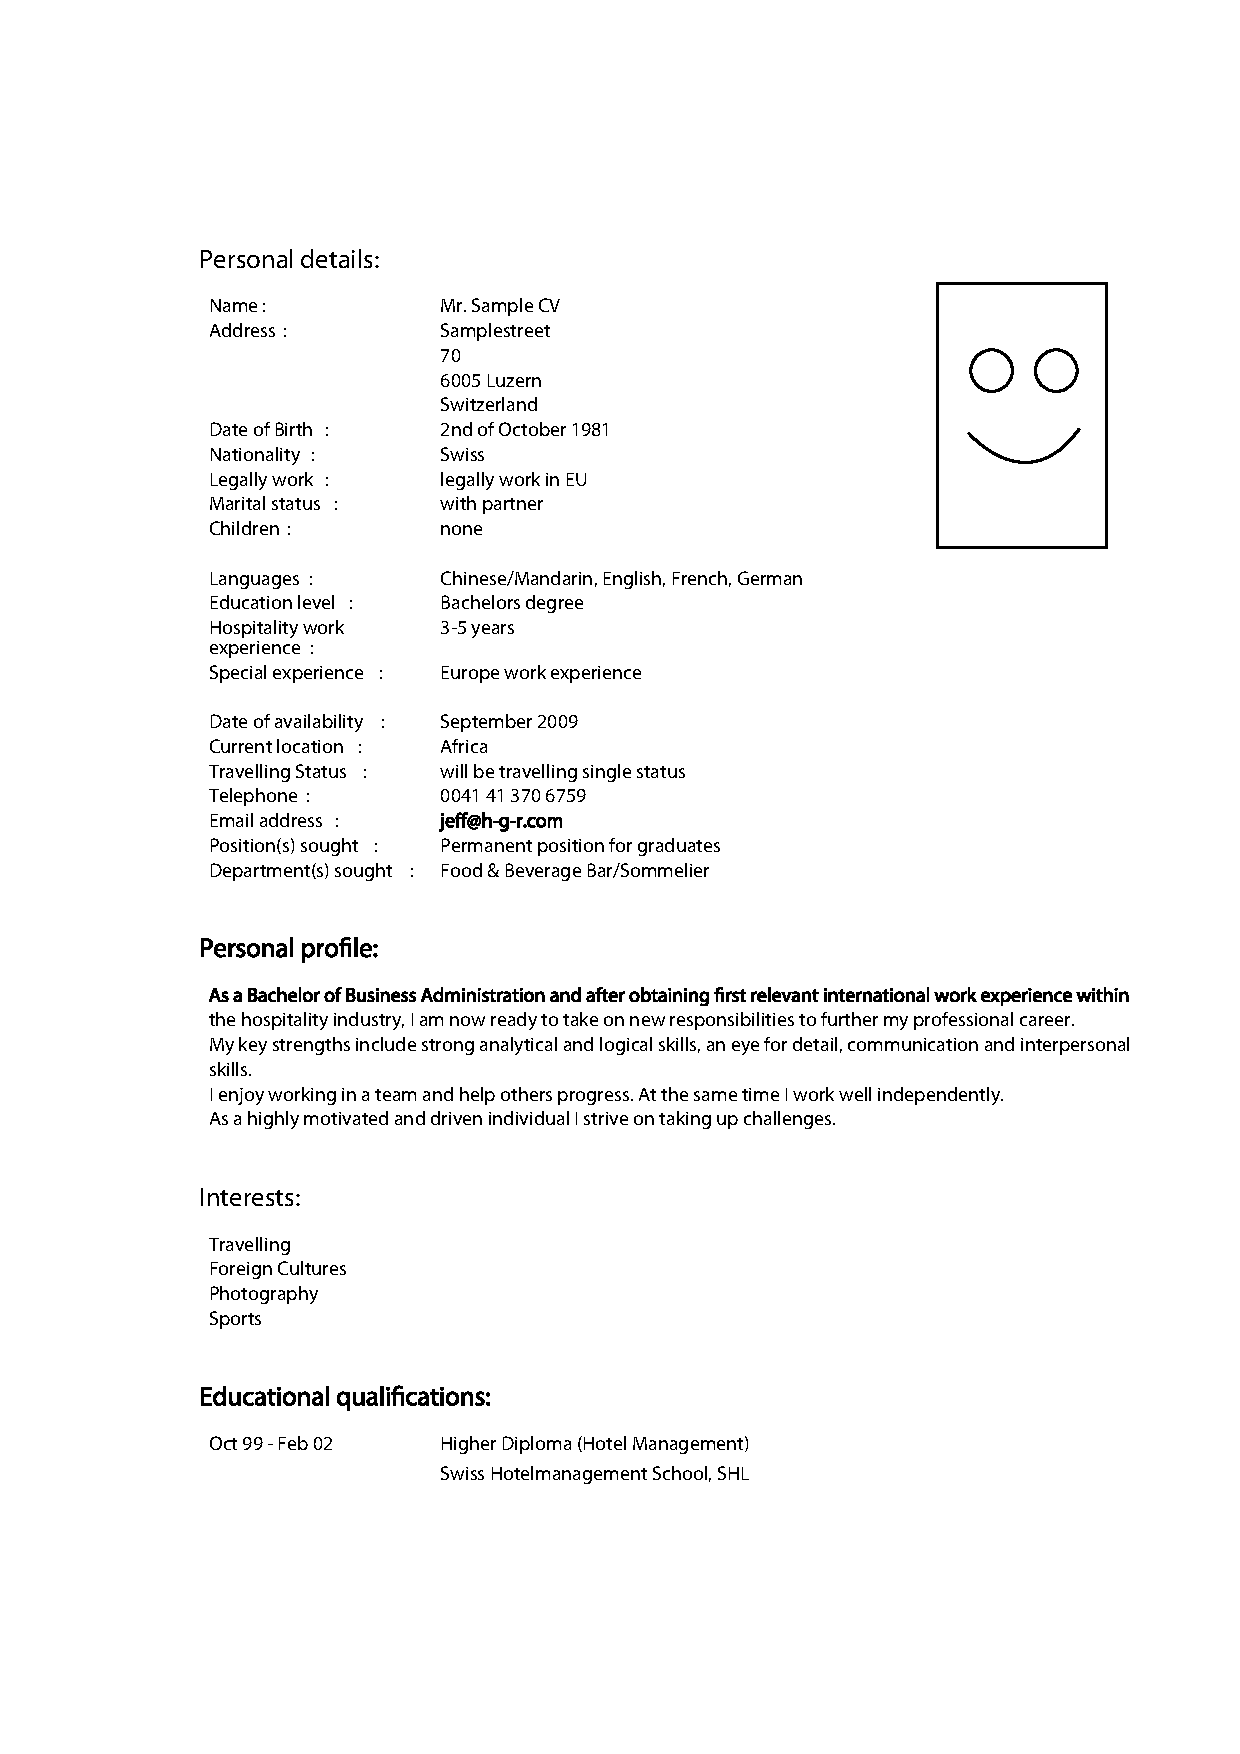
\includepdf[pagecommand=\thispagestyle{addpagenumbersforpdfimports},pages=-]{tail/cv.pdf}

\end{document}
